\documentclass[conference]{IEEEtran}
\usepackage[T1]{fontenc}
\usepackage{graphicx}
\usepackage{booktabs}
\usepackage{amsmath}
\usepackage{cite}
\usepackage{url}

\begin{document}

\title{Recording Domain, Not Code-Mixing: Closing the Generalisation Gap of
Audio Deepfake Detection on Hindi--English Telephone Speech}
% \author{...}

\maketitle

\begin{abstract}
Audio deepfake detectors report error rates below one percent on English
benchmarks. We ask what that means for Hindi--English code-mixed speech over a telephone
line, where voice fraud happens. A wav2vec~2.0 detector trained on ASVspoof 2019 LA reaches
0.85\% equal error rate (EER) on English, but 48.21\% on clean code-mixed speech and
58.42\% over a simulated narrowband channel: it rejects genuine speakers (94.8\% of
genuine Hindi--English speech) rather than missing clones. A language-controlled test on
183 unseen speakers shows code-mixing is not the cause, since genuine English is rejected
as often as mixed speech. Low-rank adaptation of the encoder (1.13\% of the parameters) on
speaker-disjoint code-mixed speech and clones lowers channel-matched error to 2.75\%. The
largest further gains come from more genuine voices and real codec audio: with 248
speakers and both simulated G.711 and real AMR-NB audio, error on unseen Tortoise clones
over AMR-NB falls from 36.3\% to 6.0\% (five seeds, no unseen-tool audio in training). A
larger encoder (SSL-AASIST) trained the same way is far better still (five seeds each,
exact tests): 0.5\% on unseen Tortoise over AMR-NB and 12.9\% on a third unseen generator,
Chatterbox, but IndicF5 stays at 15.8\% over G.711 and 21.8\% over AMR-NB. The limits are measured too:
spontaneous speech is rejected; over the simulated channel the earlier deployed model beats
a shortcut floor of cheap signal statistics in no seed, the floors of the final systems are
not yet measured, and the larger encoder's cost on live calls is untested. The detector
runs on live calls and warns the callee about ten seconds into the speech.
\end{abstract}

% Section owners follow docs plan, Week 9. Uncomment each line once its file exists.
% Introduction (owner SK). Every figure quoted here appears with its source in
% Section~\ref{sec:results}; nothing is stated here that is not measured there.
\section{Introduction}
\label{sec:intro}

Voice cloning has become a consumer technology. A few seconds of a person's speech
is enough for a zero-shot system to produce new sentences in their
voice~\cite{casanova2024xtts,betker2023tortoise}, and voice conversion does the same
without needing a transcript~\cite{rvc2023}. The obvious criminal application is the
telephone call: a voice the victim recognises, asking for money or a code, on a line
that carries no signal of who is really speaking.

Detection research has answered with strong results. On ASVspoof 2019
LA~\cite{todisco2019asvspoof}, self-supervised speech representations fine-tuned for
anti-spoofing reach error rates below one percent~\cite{tak2022wav2vec}. Our own
replication of that recipe reaches \textbf{0.85\% EER} on the evaluation partition.

That number is measured on English studio speech. The people most exposed to voice
fraud are not speaking English studio speech. In India, everyday conversation is
routinely \emph{code-mixed} --- Hindi and English alternating inside a single utterance
--- and it arrives over a narrowband telephone channel. This paper asks what happens
to a detector when both of those change at once, and what it costs to fix.

\subsection{The gap, and why it is not obvious}

The same checkpoint that scores 0.85\% EER on English scores \textbf{48.21\% EER on
clean code-mixed speech and 58.42\% over a simulated telephone channel}
(Section~\ref{sec:gap}). Over the channel its AUC is 0.381: below chance, meaning
the clones look \emph{more} genuine to it than the real speakers do.

The failure is not a mild degradation and it is not symmetric. At a 0.5 threshold
this model rejects 0.37\% of genuine English and 94.8\% of genuine Hindi--English ---
a 256-fold rise in the false-alarm rate on real speech. It has not become a weaker
detector of clones so much as a system that has stopped recognising real speakers.

Is it the code-mixing? A language-controlled test settles this. For 183 speakers
never used in training or testing, we take all-English, all-Hindi and mixed clips from
the \emph{same} lecture recordings, so only the language changes. The English-trained
detector rejects their genuine English as often as their mixed speech (84.3\% and
78.1\% on clean audio), and no amount of mixing, measured by the Code-Mixing Index,
predicts its score (Section~\ref{sec:res-language}). The gap is a recording-domain gap
that code-mixed telephone speech carries, not a property of the language mix, and
that is why adapting on in-domain audio can close it.

\subsection{Measuring against a floor, not against zero}

A low error rate on a code-mixed test set is easy to obtain for the wrong reason. If
the real and cloned clips differ in loudness, bandwidth, or recording room, a model
can separate them without learning anything about synthesis, and the resulting
number looks like detection.

We therefore report every result beside a \textbf{shortcut floor}: the error rate
eight cheap signal statistics reach on the same clips. A result better than its floor
is evidence that the model found something a trivial classifier could not; a result
at or above its floor is not evidence of anything. This discipline changes the
conclusions of this paper more than once --- including one of our own headline
conditions, which fails it.

\subsection{Contributions}

\begin{enumerate}
  \item \textbf{A measured gap.} The English-trained detector fails on code-mixed
    speech at 41.67--48.21\% EER clean and 44.15--58.42\% over the channel, far above
    every shortcut floor, with the failure characterised as a
    rejection of genuine speech rather than a loss of sensitivity to clones
    (Section~\ref{sec:gap}), and traced on a language-controlled set of 183 unseen
    speakers to the recording domain rather than to code-mixing
    (Section~\ref{sec:res-language}).
  \item \textbf{A cheap closure.} Low-rank adapters~\cite{hu2022lora} over a frozen
    wav2vec~2.0 encoder~\cite{baevski2020wav2vec}, training \textbf{1.13\% of the
    parameters}, bring channel-matched code-mixed error to \textbf{2.75\% EER}
    (3.27\% $\pm$ 1.17 over five training seeds) while retaining 2.42\% on clean
    English (Section~\ref{sec:systems}).
  \item \textbf{Matched shortcut floors.} Every detector is compared with a floor of
    eight cheap signal statistics fitted on its own training data and scored on its
    own clips, by a paired bootstrap over speakers. A floor fitted on the unseen tool
    itself would have understated the deployed detector (25.79\% against a matched
    37.79\% on Tortoise over the channel), and clip-level intervals would have
    overstated several of our own results (Section~\ref{sec:floor}).
  \item \textbf{An honest generalisation result.} Against a cloning tool no model was
    ever allowed to see, the adapters generalise on clean audio (5.44\% EER against a
    29.49\% floor). Over the telephone channel the deployed model averages 35.59\%
    across five training seeds against a 37.79\% floor and beats it in \emph{no} seed
    at the speaker level; full fine-tuning on a single attack family stays below its
    floor in every seed (19.72\%). Randomising the recording cues during training
    lowers the deployed recipe to 26.63\% over five seeds, which we report as
    exploratory (Section~\ref{sec:variants}). We report the weak result as
    prominently as the strong one.
  \item \textbf{Adaptation beats full fine-tuning where it matters.} Training the
    whole encoder on the same data reaches the lowest seen-tool error in the study
    (0.83\%) and collapses to chance on English. The adapters keep both.
  \item \textbf{A deployed system, not an illustration.} The detector runs on a live
    call and warns the callee --- and only the callee --- roughly ten seconds into
    the speech, using the same windowing and operating point the evaluation uses
    (Section~\ref{sec:system}).
\end{enumerate}

The corpora, attacks, manifests, configurations and per-clip scores behind every
number are committed, and each result table names the file it was read from.
   % SK
% Related work (owner SK). Only sources actually consulted and cited in refs.bib
% appear here; the scope limits of this survey are stated rather than hidden.
\section{Related Work}
\label{sec:related}

\subsection{Anti-spoofing benchmarks and their language}

ASVspoof 2019 LA~\cite{todisco2019asvspoof} is the reference benchmark for logical
access attacks and the training source for our Stage-1 system. It is English, read
in studio conditions, and its attacks are the text-to-speech and voice conversion
systems of its era. Its influence is what makes the question in this paper worth
asking: a field that tunes against one language in one recording condition can
mistake in-domain accuracy for detection ability.

\subsection{Self-supervised representations for detection}

The current recipe is to fine-tune a self-supervised speech encoder rather than
engineer features. wav2vec~2.0~\cite{baevski2020wav2vec} learns from unlabelled audio
and transfers well to spoofing detection, where using it as a front-end gives large
gains over hand-designed features~\cite{tak2022wav2vec}. We adopt that architecture
directly: a wav2vec~2.0 encoder with attentive statistics
pooling~\cite{okabe2018attentive} and a linear classifier.

What this literature does not settle is what the encoder's transfer depends on. Our
probing results (Section~\ref{sec:probe}) find the decision forming within the first
three layers, before linguistic representation exists --- which is consistent with a
detector reading low-level synthesis artefacts, and is why a change of channel hurts
it more than a change of language.

\subsection{Parameter-efficient adaptation}

LoRA~\cite{hu2022lora} adapts a frozen model through low-rank updates, training a
small fraction of the parameters. It is normally motivated by cost. Our results
suggest a second reason to prefer it here: with 1.13\% of parameters trainable, the
adapted model gains code-mixed performance \emph{and keeps} English, whereas
fine-tuning the whole encoder on identical data reaches a better seen-tool error and
loses English almost entirely (Section~\ref{sec:systems}). Restricting capacity
appears to limit catastrophic forgetting in a way that matters for deployment.

\subsection{The attacks}

We generate attacks rather than reuse a fixed attack set, because the code-mixed
attacks we need do not exist as a benchmark. XTTS-v2~\cite{casanova2024xtts} provides
zero-shot cross-lingual cloning from a few seconds of reference audio;
RVC~\cite{rvc2023} provides voice conversion, which changes speaker identity while
preserving the original delivery and therefore probes a different cue;
Tortoise-TTS~\cite{betker2023tortoise} is held out entirely and used only as an
unseen tool at evaluation. AffectDF~\cite{affectdf2026} informs our attack taxonomy
and reporting format.

\subsection{Code-mixed speech resources}

MUCS 2021~\cite{diwan2021mucs} supplies the Hindi--English speech this work is built
on. Code-mixed corpora are scarce relative to monolingual ones, which is itself part
of the problem this paper describes: the detector cannot be evaluated on a language
setting for which no evaluation data has been assembled.

\subsection{What this survey does not cover}

This is a targeted review of the work our system is built from, not a complete
survey of audio deepfake detection. In particular we do not review the wider
countermeasure literature beyond the self-supervised line, nor the speaker
verification literature that anti-spoofing was originally developed to protect, nor
detection for languages other than English and Hindi--English. We also found no
prior work measuring detector generalisation to code-mixed speech over a telephone
channel; we state that as the gap we address rather than as a claim of novelty we
can prove exhaustively.
   % SK
% Dataset, channel protocol and ethics (owner L). Complements Section~\ref{sec:method},
% which gives the attack and split tables; this section covers composition, the
% speaker-pool discipline, exclusions, and what may be released.
% Sources: docs/datasheet.md, docs/licences.md, docs/results/dataset_inventory_v1.md
\section{Data}
\label{sec:dataset}

\subsection{Composition}

The code-mixed side is built from two corpora, indexed clip by clip with durations
measured from the audio rather than estimated:

\begin{itemize}
  \item \textbf{MUCS 2021 Hindi--English}~\cite{diwan2021mucs}: 52{,}825 clips,
    89.5 hours, 520 speakers. Lecture and read speech, code-mixed at the utterance
    level. This is the bonafide pool and the source of every cloning reference.
  \item \textbf{HiACC, adult subset}: 3{,}318 clips, 3.2 hours, 24 speakers.
    Spontaneous speech, used for evaluation only.
\end{itemize}

Together 56{,}143 clips and 92.8 hours over 544 speakers. The English side is
ASVspoof 2019 LA~\cite{todisco2019asvspoof}: 121{,}461 clips and 109.6 hours across
the official train, development and evaluation partitions, at a spoof-to-real ratio
of 8.7:1.

That ratio matters when reading results across the two. The code-mixed evaluation
sets are close to balanced, near 1.5:1, so the same detector confidence produces
different operating points on the two families and accuracy figures are not directly
comparable between them.

\subsection{Speaker pools, frozen before any audio was generated}

The 520 MUCS speakers are divided once into three disjoint pools --- 25 for training,
10 for adaptation, 15 for evaluation --- and the division was committed before a
single clip was cloned. This ordering is the point: a pool drawn after seeing which
speakers clone well would quietly select for them.

The original study used 50 of the 520 speakers. For the extension experiments the
remaining speakers with enough clips were carved, again before any of their audio was
scored or cloned, into three further pools whose membership is committed and hashed:
\emph{new test speakers} (60), \emph{language control} (183, evaluation only) and
\emph{extra adaptation} speakers (227). The two evaluation pools are added to the
leakage checks, so no configuration can train on them.

Disjointness is enforced mechanically rather than by discipline.
\texttt{tests/test\_splits.py} fails the build if a speaker crosses a pool boundary,
if a held-out tool reaches a training manifest, or if any excluded identifier appears
anywhere. The anti-leakage checks run before every training launch.

\subsection{Who the models hear, and who they are tested on}
\label{sec:data-speakers}

Table~\ref{tab:speakers} counts speakers per set. Adaptation uses 8 speakers for
training and 2 for development. Models that train on RVC also hear the 13 source
speakers of the RVC training half, drawn from the training pool, so the deployed model
trains on 21 speakers. Its test sets hold 15 + 12 speakers it never heard, and HiACC
adds 24 more, speaking spontaneously rather than reading.

\begin{table}[t]
\centering
\caption{Speakers per set. No test speaker appears in any training set.}
\label{tab:speakers}
\small
\begin{tabular}{@{}lrr@{}}
\toprule
Set & Clips & Speakers \\
\midrule
Training, XTTS only                & 2{,}154 & 8 \\
Training, XTTS + RVC (deployed)    & 2{,}854 & 21 \\
Training, extended (Sec.~\ref{sec:data-extension}) & 8{,}018 & 248 \\
Development                        & 506     & 2 \\
\midrule
Evaluation pool / CM04 (read)      & 3{,}966 / 2{,}024 & 15 \\
RVC test (read)                    & 619     & 12 \\
HiACC adult (spontaneous, genuine) & 3{,}318 & 24 \\
\midrule
New test speakers (CM05 + CM06)    & 4{,}392 & 60 \\
IndicF5 test (CM07)                & 1{,}177 & 54 \\
Chatterbox test (CM09)             & 1{,}176 & 61 \\
Language control (genuine)         & 1{,}290 & 183 \\
\bottomrule
\end{tabular}
% docs/results/hiacc_false_alarm_v1.md; experiments/results/floor_v2/per_speaker_eer.csv
\end{table}

\subsection{Different voices, different speaking style}
\label{sec:data-styles}

A pooled EER hides how unevenly the error falls on speakers. For the deployed model
over the channel, per-speaker EER on the seen tool runs from 0.0\% to 11.0\% (median
0.7\%), and on the unseen Tortoise attack from 6.4\% to 45.5\% (median 28.1\%), with 6
of the 15 speakers above their own shortcut floor.

Spontaneous speech is a harder test still. HiACC holds genuine speech only, so we
measure false alarms: the share of genuine clips called fake at the deployed operating
point. On the MUCS read lectures of the evaluation pool the deployed model calls
0.89\% [0.54, 1.29] of genuine clips fake; on HiACC's 24 spontaneous speakers it calls
54.37\% [44.43, 64.15] fake, a difference of 53.5 points, with every speaker above
10\% (13.9--89.5\%). Clip length does not explain it: longer HiACC clips are rejected
more often than short ones. Adaptation moved the detector's notion of genuine speech
to the lecture recordings it was adapted on, not to Hindi--English speech in general.
HiACC differs from MUCS in recording conditions as well as in speaking style, and this
test cannot say which of the two drives the false alarms.

\subsection{Attacks}

No benchmark supplies code-mixed deepfakes, so they were generated. Each generator
ran from a job table committed \emph{before} the run, so what was generated is
decided in version control rather than on a GPU, and every clip carries its speaker,
transcript and seed.

Quality screening rejects stalled, near-silent and clipped output. Pass rates were
99.95\% for the XTTS-v2~\cite{casanova2024xtts} training attack, 93.6\% for
RVC~\cite{rvc2023} conversion, and 91.6\% for the held-out
Tortoise-TTS~\cite{betker2023tortoise} attack. The Tortoise failures are concentrated
in one speaker, who drops from 34 clips to 15 usable while every other speaker keeps
at least 30 --- a reference-quality problem for that speaker rather than a property
of the tool.

The held-out attack is held out completely. No model in this study is trained on
Tortoise audio, and no training manifest may contain it.

\subsection{Extension: new speakers, a second unseen tool, more training voices}
\label{sec:data-extension}

Five further attack sets were made the same way, each from a committed job table:

\begin{itemize}
  \item \textbf{CM05}, XTTS-v2 clones of the 60 new test speakers: 1{,}770 of 1{,}800
    clips pass screening (98.3\%). It tests the seen tool on unseen people.
  \item \textbf{CM06}, Tortoise clones of the same 60 speakers: 222 of 240 (92.5\%).
  \item \textbf{CM07}, clones by IndicF5~\cite{ai4bharat2025indicf5}, a flow-matching
    Indian-language TTS built on F5-TTS~\cite{chen2024f5tts}, from all-Hindi references
    and all-Hindi sentences of other speakers: 526 of 610 (86.2\%); most rejections
    stall at two to six characters a second. Like Tortoise it never enters training;
    it is the second unseen tool and the most recent generator in the study.
  \item \textbf{CM08}, XTTS-v2 clones of the 227 extra adaptation speakers: 1{,}759 of
    1{,}816 (96.9\%), used only for training.
  \item \textbf{CM09}, clones by Chatterbox Multilingual (Resemble AI, MIT licence), a
    recent multilingual cloner, from the same references and sentences as CM07, so the
    two sets pair clip for clip: 525 of 610 (86.1\%); 78 of the 85 rejections stall at
    five characters a second or less. It is a third unseen tool and never enters
    training. Chatterbox embeds an imperceptible watermark in everything it writes; we
    keep its output as generated and note that a detector could in principle use it.
\end{itemize}

Predicted naturalness separates the tools. UTMOS~\cite{saeki2022utmos}, a predictor of
the mean opinion score, gives IndicF5 clones 3.07 [2.99, 3.15] against 3.10 [3.01, 3.18]
for the same speakers' genuine all-Hindi speech, a difference within noise; XTTS-v2 sits
half a point below its genuine speech (2.66 against 3.17) and Tortoise lower still
(2.48), on 200 clean clips per set. Of the three tools scored, the newest, IndicF5, is
also the most natural (Chatterbox and RVC were not scored).

Genuine counterparts come from the same speakers: 2{,}400 clips of the new test
speakers, 651 all-Hindi clips of the IndicF5 speakers and 3{,}405 clips of the extra
adaptation speakers. Every clip passes through the same level normalisation and
telephone channel as the original sets. With CM08 and the extra genuine clips, an
extended training set grows from 21 to 248 genuine speakers (8{,}018 clips) without
touching any test pool.

\subsection{A language-controlled test set}
\label{sec:data-control}

To separate the language from the recording, each genuine clip of the 183 control
speakers is tagged word by word from its transcript, where MUCS writes Hindi in
Devanagari and English in Latin script. A clip is \emph{all English} or \emph{all
Hindi} when every tagged word is in one language (at least three words), and
\emph{mixed} when its Code-Mixing Index~\cite{das2014cmi} is at least 20. Every
speaker with an all-English clip contributes all of them plus equally many all-Hindi
and mixed clips from the same lecture recordings: 439, 412 and 439 clips. Speaker,
recording and channel are held fixed; only the language changes.

\subsection{The telephone channel}

The channel condition is a simulated narrowband chain: resample to 8~kHz, G.711
$\mu$-law encode and decode, additive noise at 20~dB SNR, resample back.

It was validated by measurement rather than assumed. Energy above 4~kHz falls from
0.185\% to 0.0001\% of total energy, and the measured SNR matches the requested one.
Clean and channel copies of every evaluation set are retained separately, so the
channel effect stays separable from the language effect throughout the results.

G.711 is the fixed-line codec and nearly transparent; mobile calls are carried by AMR-NB,
which models the voice and discards the rest. As a check on the simulation, the
new-speaker, IndicF5 and CM04 sets are also passed through the reference AMR-NB
encoder at 12.2~kbit/s and decoded back, with no added noise, so that condition isolates
a real mobile codec.

\subsection{Exclusions and ethics}

\textbf{Child audio is excluded entirely.} HiACC ships 5{,}176 files of which 1{,}858
are children. They are quarantined on extraction and are never used as bonafide
material, never as a cloning reference, and never as evaluation data.

This is reported in detail because it failed once. An automatic quarantine silently
did not run, and the child folder sat live in the corpus until it was caught by
hand-verification against the real folder layout --- not by the code that was
supposed to prevent it. After the fix the preprocessing reaches exactly 3{,}318 adult
files and no child identifier appears in any manifest. The lesson we record is that a
quarantine nobody audits is a quarantine that is not running.

\textbf{The generated audio is not released.} It is cloned speech of identifiable
people and this project's repository is public. The clones are held privately, while
per-clip metadata, the job tables and SHA-256 checksums are committed, so the corpus
is auditable without the audio being distributed.

\textbf{Licensing constrains what a release could contain.} MUCS is CC BY-SA 4.0, so
clones derived from MUCS references inherit ShareAlike. HiACC is CC BY 4.0, ASVspoof
is under its own research licence, and one surveyed corpus is non-commercial only.
Any future release of the code-mixed spoof set must satisfy the strictest of these.

\subsection{What the composition cannot tell us}

The headline gap is \emph{English studio speech to Hindi--English lecture speech},
because that is what the two corpora are, and language and recording domain move
together across them. The language-controlled set (Section~\ref{sec:data-control})
separates the two within MUCS, and Section~\ref{sec:res-language} shows the gap
follows the recording rather than the language mix. It cannot speak for other
recording conditions: all of its clips are read lectures, and spontaneous speech
(HiACC) still differs in both style and recording.
        % L: dataset, channel protocol, ethics
% Methodology (owner M). Every number below is read from a committed config,
% manifest or results file; the source is named in a comment beside it.

\section{Methodology}
\label{sec:method}

\subsection{Three systems}
\label{sec:systems}

We compare three detectors that share one architecture and differ only in what
they are trained on and which weights move.

\begin{itemize}
  \item \textbf{S1, English only.} Trained on ASVspoof 2019 LA~\cite{todisco2019asvspoof}
        and nothing else. It is the conventional detector whose transfer to
        code-mixed speech we measure.
  \item \textbf{S2, LoRA adaptation.} S1 with low-rank adapters~\cite{hu2022lora}
        trained on code-mixed Hindi--English data. The encoder weights of S1 stay
        frozen, so S2 can be read as S1 plus a small correction.
  \item \textbf{S3, native training.} The same architecture fine-tuned end to end on
        exactly the code-mixed manifests used by the matching S2 run, starting from
        the self-supervised checkpoint and never from S1. It shows what the
        code-mixed data alone supports.
\end{itemize}

S2 and S3 are each trained in four variants: on XTTS clones only or on XTTS clones
plus RVC conversions, and on clean audio or on channel-matched audio
(Sec.~\ref{sec:channel}). This gives eight code-mixed models and one English model.

\subsection{Data}
\label{sec:data}

\textbf{English.} ASVspoof 2019 LA~\cite{todisco2019asvspoof}: the official training
partition for S1, and the official evaluation partition of 71{,}237 clips over
attacks A07--A19 for English retention.

\textbf{Code-mixed real speech.} Hindi--English code-switched lecture speech from the
MUCS 2021 corpus~\cite{diwan2021mucs}. Speakers are divided into disjoint pools
before any synthesis: an adaptation pool of 10 speakers, used only by S2 and S3,
and an evaluation pool of 15 speakers, never seen in training.
% configs/data/splits.yaml; docs/datasheet.md

\textbf{Code-mixed synthetic speech.} Four attack sets are built from these pools
(Table~\ref{tab:attacks}). XTTS-v2~\cite{casanova2024xtts} zero-shot clones are made
for both pools, so at test time XTTS is a \emph{seen tool on unseen speakers}.
RVC~\cite{rvc2023} converts one MUCS speaker into another. Its conversions are split
by speaker so that neither the source nor the target speaker of any training
conversion appears in the RVC test half. Tortoise-TTS~\cite{betker2023tortoise}
clones of the evaluation pool form the held-out attack: by rule it never appears in
any training manifest, and an automated test fails the build if it does.
% tests/test_splits.py, tests/test_config_guard.py

\begin{table}[t]
\centering
\caption{Code-mixed attack sets. Usable clips passed the quality screen.}
\label{tab:attacks}
\small
\begin{tabular}{@{}llrl@{}}
\toprule
Set  & Tool      & Usable  & Role \\
\midrule
CM01 & XTTS-v2   & 3{,}998 & test, seen tool \\
CM02 & RVC       & 1{,}404 & split: train half, test half \\
CM03 & XTTS-v2   & 1{,}600 & adaptation only \\
CM04 & Tortoise  & 458     & test, unseen tool \\
\bottomrule
\end{tabular}
% docs/datasheet.md
\end{table}

\begin{table}[t]
\centering
\caption{Code-mixed training and test sets (clips).}
\label{tab:splits}
\small
\begin{tabular}{@{}lrrr@{}}
\toprule
Set & Real & Fake & Total \\
\midrule
Adaptation, XTTS only   & 874     & 1{,}280 & 2{,}154 \\
Adaptation, XTTS + RVC  & 1{,}217 & 1{,}637 & 2{,}854 \\
Adaptation dev          & 186     & 320     & 506 \\
\midrule
Eval pool (XTTS)        & 1{,}566 & 2{,}400 & 3{,}966 \\
CM04 (Tortoise)         & 1{,}566 & 458     & 2{,}024 \\
RVC test\textsuperscript{a} & 302     & 317     & 619 \\
\bottomrule
\multicolumn{4}{@{}l}{\footnotesize \textsuperscript{a}Real side: MUCS source clips of the held-out speakers.}
\end{tabular}
% data/manifests/codemix_adapt_*.csv, codemix_eval.csv; results/w10/*.json
\end{table}

\textbf{Preprocessing.} All audio is resampled to 16~kHz mono, trimmed by voice
activity detection and kept between 2 and 10~s. Every clip is level-normalised to
$-23$~dBFS RMS. This step matters: without it the XTTS clones arrive
peak-normalised while the lecture audio does not, and signal level alone separates
the classes (Sec.~\ref{sec:floor}).
% configs/data/channel_sim.yaml (preprocess block); docs/results/bundle_normalisation_v1.md

\subsection{Channel-matched condition}
\label{sec:channel}

The target application is a telephone call. We therefore render every clip through a
narrowband telephony chain: resample from 16 to 8~kHz, encode and decode with G.711~\cite{itu1988g711}
$\mu$-law, add white noise at 20~dB SNR and resample back to 16~kHz. Noise is seeded
per clip from a hash of its name. A single shared noise draw would add one identical
waveform to every clip, which a detector could learn in place of the speech. On the
evaluation render, energy above 4~kHz falls from 0.185\% to 0.0001\% and the measured
SNR is 18.8~dB. A model is always scored in the condition it was trained in.
% configs/data/channel_sim.yaml; docs/results/channel_matched_v1.md

\subsection{Model}
\label{sec:model}

The detector is a wav2vec~2.0 base encoder~\cite{baevski2020wav2vec} followed by
attentive statistics pooling~\cite{okabe2018attentive} and a two-layer classifier.
The encoder reads the raw 16~kHz waveform. Seven convolutional layers produce one
768-dimensional frame every 20~ms, each covering 25~ms of audio, and twelve
transformer layers contextualise the frames. Pooling computes an attention-weighted
mean and standard deviation over frames (attention width 128), giving a
1{,}536-dimensional vector. The classifier is Linear(1536, 256), ReLU, dropout 0.3 and
Linear(256, 2); its softmax output is read as $P(\text{genuine})$. The model has
95{,}454{,}083 parameters. In every system the convolutional feature extractor is
frozen, following common practice for self-supervised
anti-spoofing~\cite{tak2022wav2vec}.
% src/models/{encoder,pooling,classifier,detector}.py

\subsection{Training}
\label{sec:training}

All systems use AdamW~\cite{loshchilov2019adamw} with weight decay $10^{-5}$, 4~s training crops, mixed
precision and seed 1234. The remaining settings are in Table~\ref{tab:hparams}.
The checkpoint with the lowest EER on the development set is kept.

\textbf{S2.} Rank-8 adapters ($\alpha = 16$, dropout 0.05) wrap the query, key,
value and output projections of all twelve transformer layers. Only the adapters and
the classifier head are trained: 1{,}082{,}371 parameters, or 1.13\% of the model.
% src/models/lora.py; docs/results/gap_closure_v1.md

\textbf{S2 and S3} use class-weighted cross-entropy, since the adaptation sets are
not balanced (Table~\ref{tab:splits}).

\begin{table}[t]
\centering
\caption{Training settings.}
\label{tab:hparams}
\small
\begin{tabular}{@{}lccc@{}}
\toprule
                 & S1 & S2 (LoRA) & S3 (native) \\
\midrule
Initialised from & wav2vec 2.0 & S1 & wav2vec 2.0 \\
Trained weights  & transformer, head & adapters, head & transformer, head \\
Learning rate    & $10^{-5}$ & $10^{-4}$ & $10^{-5}$ \\
Batch size       & 4 & 8 & 8 \\
Epochs           & 3 & 5 & 10 \\
Training data    & ASVspoof LA & code-mixed & code-mixed \\
\bottomrule
\end{tabular}
% configs/train_stage1_run.yaml, train_lora_norm_*.yaml, train_s3_native_*.yaml
\end{table}

\subsection{Evaluation}
\label{sec:eval}

We report equal error rate (EER) and area under the ROC curve (AUC), scoring one
deterministic 4~s crop per clip, with 95\% bootstrap confidence intervals over
clips~\cite{efron1993bootstrap}. Clips from one speaker are not independent and each
test set holds only 12--15 speakers, so every comparison between two systems, or
between a system and its floor, is made on a paired bootstrap that resamples whole
speakers (1{,}000 resamples), never by setting two separately computed intervals side
by side.
Three code-mixed test sets probe three kinds of generalisation: the evaluation pool
(seen tool, unseen speakers), CM04 (unseen tool) and the RVC test half (speakers
unseen as either source or target). The ASVspoof 2019 LA evaluation set measures
what each code-mixed model retains of English.

\subsubsection{Shortcut floor}
\label{sec:floor}
A low EER on a newly built corpus is not evidence by itself. The real and fake halves
come from different pipelines, and pipeline provenance can separate them without any
knowledge of synthetic speech. Following the check proposed with
AffectDF~\cite{affectdf2026}, we fit a logistic regression on eight cheap signal
statistics (RMS mean and standard deviation, peak amplitude, clipping ratio, DC
offset, zero-crossing rate, spectral roll-off and high-frequency energy ratio). Its
EER is the \emph{shortcut floor}. Each detector gets its own floor: the regression is
fitted on exactly the manifest the detector was trained on and scored on exactly the
clips the detector is scored on, so the two differ only in what they can hear. A
result counts as evidence only when the paired, speaker-resampled 95\% interval of
EER(detector)~$-$~EER(floor) lies entirely below zero; an interval that contains zero
is reported as inconclusive.

\textbf{Reading the floor.} The floor is a reference, not a bound on what can be
achieved. A detector below its floor uses information beyond the eight statistics,
which rules out the cheapest explanation for its score but does not show that it
ignores recording provenance: an encoder of 95M parameters can exploit subtler
domain cues, such as room, microphone, noise or pause structure, that the eight
statistics do not measure. A detector at or above its floor is not shown to rely on
the shortcut either; its result simply carries no evidence of learning beyond it.

An earlier version of this check fitted the CM04 floor on half of CM04 itself,
Tortoise clips included, and scored it on the other half. That regression has seen
the attack the detectors never see. We keep its value as an \emph{oracle floor}, the
separation recording cues reach given labelled examples of the unseen tool, and
report it beside the matched floor.
% src/data/lowlevel_cue.py, src/training/floor_compare.py
% experiments/results/floor_compare_v2.json; docs/results/shortcut_floor_v2.md
      % M
% Experiments and Results (owner M). Sources:
%   experiments/results/systems_s1_s2_s3.json  (every S2/S3 cell, CIs, floors)
%   experiments/asvspoof_retention_summary.json (S1 English)
%   results/s1_norm/stage1__*.json         (S1 on the normalised code-mixed sets)
%   experiments/results/lowlevel_cue_check_*.json (shortcut floors)

\section{Experiments and Results}
\label{sec:results}

\subsection{The generalisation gap}
\label{sec:gap}

S1 is a strong English detector. On the ASVspoof 2019 LA evaluation set it reaches
0.85\% EER (AUC 0.994) over attacks it never saw in training; an independent
re-scoring of the same checkpoint on the same 71{,}237 clips gives 0.90\%
[0.83, 0.99]. On the same
code-mixed sets that S2 and S3 are measured on, it fails every one
(Table~\ref{tab:gap}): 41.67--48.21\% EER on clean audio and 44.15--58.42\% over the
telephone channel. Every cell is above the lowest shortcut floor of its set and
condition (Table~\ref{tab:floors}), which never exceeds 29.49\% clean and 25.79\%
over the channel; no cell comes close.

\begin{table}[t]
\centering
\caption{S1, trained on English only, on the normalised code-mixed sets. Floor: the
lowest shortcut floor of that set and condition in Table~\ref{tab:floors}.}
\label{tab:gap}
\small
\resizebox{\columnwidth}{!}{%
\begin{tabular}{@{}llrrr@{}}
\toprule
Test set & Condition & EER (\%) & AUC & Floor \\
\midrule
ASVspoof LA eval (English) & clean   & 0.85  & 0.994 & -- \\
\midrule
Eval pool (XTTS)           & clean   & 48.21 & 0.557 & 5.17 \\
CM04 (Tortoise)            & clean   & 41.67 & 0.597 & 29.49 \\
RVC test                   & clean   & 43.46 & 0.546 & 16.96 \\
Eval pool (XTTS)           & channel & 58.42 & 0.381 & 9.96 \\
CM04 (Tortoise)            & channel & 44.15 & 0.561 & 25.79 \\
RVC test                   & channel & 55.57 & 0.425 & 20.52 \\
\bottomrule
\end{tabular}%
}
% results/s1_norm/stage1__*.json
\end{table}

The AUCs show how it fails. S1 does not mainly miss the fakes; it rejects the real
speakers. It calls 94.8\% of genuine Hindi--English speech fake on clean audio, with
a median $P(\text{genuine})$ of 0.0005. The same model at the same operating point
rejects 0.37\% of genuine English, so changing the language and the recording domain
raises its false-alarm rate on real speech by a factor of 256.
Over the telephone channel every AUC falls
below 0.5, so the clones look \emph{more} genuine to S1 than the real speakers do.
In a deployment this is the more damaging error: nearly every genuine caller would
be flagged. The model's notion of genuine speech is tied to the recording conditions
and language of its training data rather than to properties of synthesis. Because
ASVspoof is studio read speech and MUCS is lecture audio, this gap combines language
shift with recording-domain shift; the next subsection separates the two.

\subsection{Code-mixing or recording domain?}
\label{sec:res-language}

The language-controlled set (Section~\ref{sec:data-control}) holds the speaker and the
recording fixed and changes only the language. If code-mixing were what fooled S1, its
false alarms would be highest on the mixed clips. They are not
(Table~\ref{tab:language}). On clean audio S1 rejects 84.3\% of genuine all-English
clips, 85.2\% of all-Hindi and 78.1\% of mixed; within the same speakers, mixed speech
is rejected 9.5 points \emph{less} often than English [$-$15.6, $-$3.5]. Over the
channel the three conditions are 43.1, 53.2 and 41.2\%, and the mixed-minus-English
difference ($-$5.2 [$-$13.4, +2.9]) contains zero. The adapted systems keep false
alarms at 2--5\% in every condition, with no condition singled out. S1 rejects English
lecture speech by the same English speakers almost exactly as often as it rejects their
code-mixed speech: the failure follows the recording, not the language mix.

\begin{table}[t]
\centering
\caption{False alarms (\%) on the language-controlled genuine set: 183 unseen speakers,
each in three language conditions from the same recordings. Last column: within-speaker
difference mixed $-$ English (points), 95\% speaker-bootstrap interval.}
\label{tab:language}
\small
\resizebox{\columnwidth}{!}{%
\begin{tabular}{@{}lrrrr@{}}
\toprule
Model, audio & English & Hindi & Mixed & Mixed $-$ English \\
\midrule
S1, clean          & 84.3 & 85.2 & 78.1 & $-$9.5 [$-$15.6, $-$3.5] \\
S1, channel        & 43.1 & 53.2 & 41.2 & $-$5.2 [$-$13.4, +2.9] \\
S2 (clean), clean  & 5.2  & 2.9  & 2.3  & $-$3.3 [$-$6.3, $-$0.6] \\
Deployed S2, channel & 4.3 & 4.1 & 2.3  & $-$2.6 [$-$5.8, +0.5] \\
\bottomrule
\end{tabular}%
}
% docs/results/language_control_v1.md
\end{table}

The evaluation pool tells the same story at the level of single clips. Grouping its
genuine clips by Code-Mixing Index, S1 rejects 94.5, 95.2, 95.1 and 93.5\% in the
bands 0--10, 10--25, 25--40 and 40--50 on clean audio, and the rank correlation
between a clip's CMI and its score is $-$0.01; over the channel it is +0.13, so more
mixing makes a clip look, if anything, slightly \emph{more} genuine
(\texttt{docs/results/cmi\_bands\_v1.md}). The gap this paper closes is therefore a
recording-domain gap that code-mixed telephone speech happens to carry, which is why
adaptation on in-domain audio closes it.

\subsection{Shortcut floors}
\label{sec:floors}

Before reading any code-mixed result we measured how far cheap statistics get on
each test set (Table~\ref{tab:floors}). On the corpus as first built, before level
normalisation, the eight statistics reached 1.39\% EER on the evaluation pool. A
headline number of 1.34\% from our first clean adapter therefore had no margin over
a logistic regression, and we withdrew it. Normalising to $-23$~dBFS raises the
floor to 5.17\%. The remaining separation comes from zero-crossing rate and RMS
variability, a trace of lecture recording set against vocoder output that
normalisation cannot remove. Every code-mixed result below is compared with the
matched floor of its own training data, set and condition (Sec.~\ref{sec:floor}).

Table~\ref{tab:floors} shows why the floor must be matched. On CM04 the eight
statistics reach 25.79\% over the channel when the regression has seen Tortoise
(the oracle floor), but only 33.64--37.79\% when it is fitted on the XTTS and RVC
data the detectors learn from: provenance cues learned from one generator transfer
to another no better than the detectors do. Comparing a detector that never saw
Tortoise with a regression that did would understate the detector.

\begin{table}[t]
\centering
\caption{Shortcut floors, EER (\%) of a logistic regression on eight signal
statistics, scored on the same clips as the detectors. \emph{Matched}: fitted on the
detector's own training data. \emph{Oracle}: fitted on half of CM04, Tortoise
included, and scored on the other half.}
\label{tab:floors}
\small
\resizebox{\columnwidth}{!}{%
\begin{tabular}{@{}llrrr@{}}
\toprule
Fitted on & Condition & Eval pool & CM04 & RVC test \\
\midrule
XTTS training data       & clean   & 5.17  & 29.49 & 17.93 \\
XTTS + RVC training data & clean   & 5.62  & 31.43 & 16.96 \\
XTTS training data       & channel & 10.01 & 33.64 & 23.91 \\
XTTS + RVC training data & channel & 9.96  & 37.79 & 20.52 \\
\midrule
Oracle (CM04 itself)     & clean   & --    & 31.21 & --    \\
Oracle (CM04 itself)     & channel & --    & 25.79 & --    \\
\bottomrule
\end{tabular}%
}
% experiments/results/floor_compare_v2.json; lowlevel_cue_check_cm04_*.json
\end{table}

\begin{figure}[t]
\centering
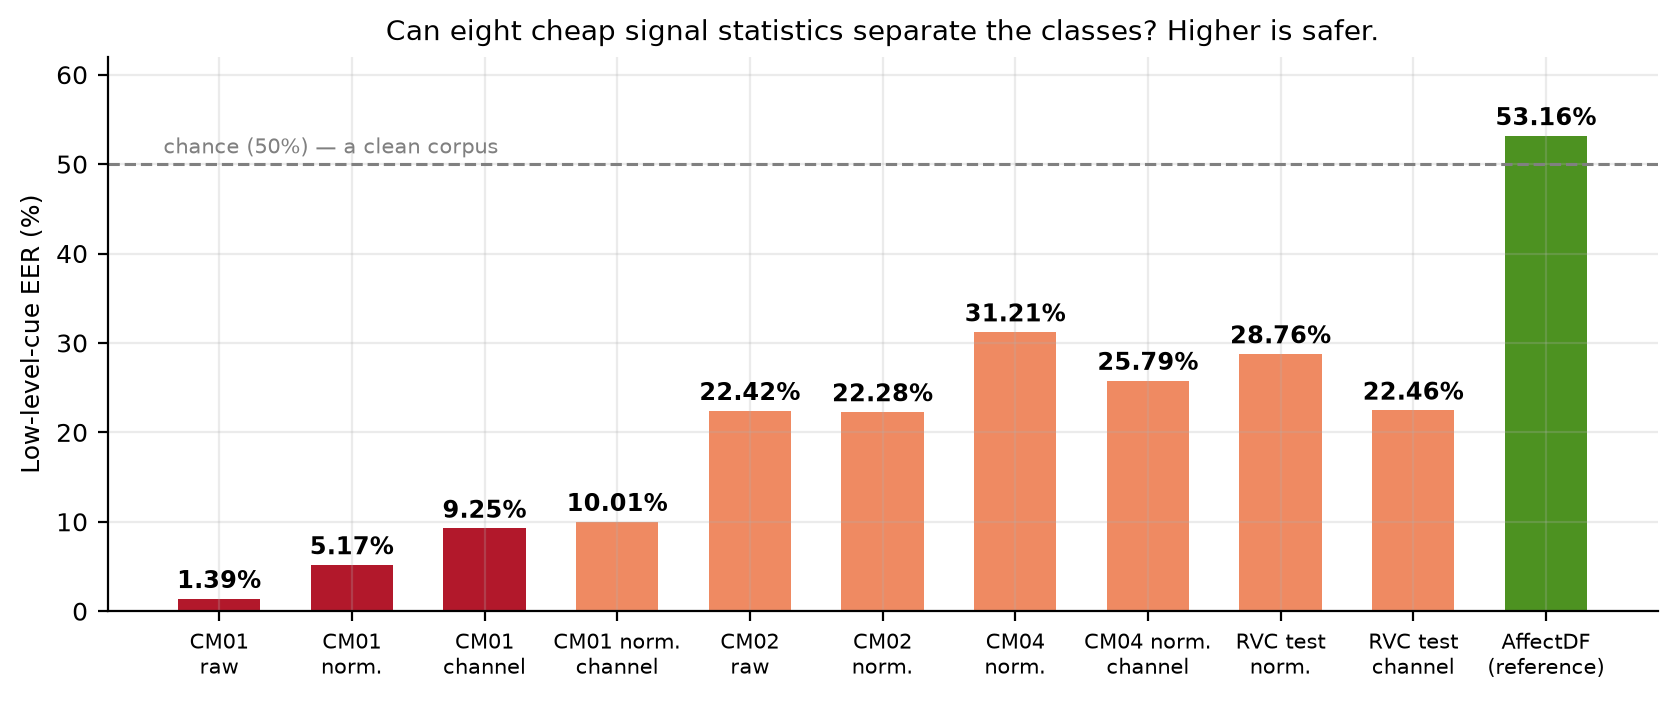
\includegraphics[width=\columnwidth]{figures/shortcut_gate.png}
\caption{Shortcut gate: EER of the eight-statistic logistic regression against
chance, per set and condition.}
\label{fig:gate}
\end{figure}

\subsection{Adaptation and native training}
\label{sec:main}

Table~\ref{tab:main} gives every S2 and S3 model on every test set, in its own
training condition, and Fig.~\ref{fig:systems} shows the same numbers against the
floors.

\begin{table*}[t]
\centering
\caption{EER (\%) with 95\% bootstrap confidence intervals over clips. Marks come from
the paired, speaker-resampled comparison with the matched floor of
Table~\ref{tab:floors}: \textbf{bold}, the whole interval of detector minus floor is
below zero (evidence of learning beyond the shortcut); \textit{italic}, the interval
contains zero (inconclusive); \textit{italic}$^\dagger$, the whole interval is above
zero (worse than the shortcut). English has no floor.}
\label{tab:main}
\small
\begin{tabular}{@{}lllcccc@{}}
\toprule
System & Training attacks & Condition & Eval pool (XTTS) & CM04 (Tortoise) & RVC test & English \\
\midrule
S2 LoRA   & XTTS       & clean   & \textbf{1.46} {\scriptsize[1.01, 1.94]} & \textbf{5.44} {\scriptsize[4.05, 6.57]}   & \textit{23.91} {\scriptsize[20.33, 27.64]} & 15.83 {\scriptsize[15.54, 16.04]} \\
S2 LoRA   & XTTS       & channel & \textit{4.41} {\scriptsize[3.78, 5.19]} & \textit{28.16} {\scriptsize[25.44, 30.20]} & \textit{29.56} {\scriptsize[26.49, 32.79]} & 2.55 {\scriptsize[2.43, 2.67]} \\
S2 LoRA   & XTTS + RVC & clean   & \textbf{1.99} {\scriptsize[1.47, 2.45]} & \textbf{12.01} {\scriptsize[10.42, 13.64]} & \textbf{5.01} {\scriptsize[3.55, 6.95]}   & 3.75 {\scriptsize[3.63, 3.91]} \\
S2 LoRA   & XTTS + RVC & channel & \textbf{2.75} {\scriptsize[2.22, 3.37]} & \textit{30.99} {\scriptsize[28.72, 33.84]} & \textbf{5.01} {\scriptsize[3.39, 6.95]}   & 2.42 {\scriptsize[2.31, 2.54]} \\
\midrule
S3 native & XTTS       & clean   & \textbf{1.46} {\scriptsize[1.08, 1.82]} & \textit{27.72} {\scriptsize[25.77, 30.14]} & \textit{45.07}$^\dagger$ {\scriptsize[40.87, 50.24]} & 56.42 {\scriptsize[55.81, 56.93]} \\
S3 native & XTTS       & channel & \textbf{1.92} {\scriptsize[1.43, 2.40]} & \textbf{13.71} {\scriptsize[12.30, 15.23]} & \textit{32.15} {\scriptsize[28.43, 35.55]} & 55.83 {\scriptsize[55.31, 56.41]} \\
S3 native & XTTS + RVC & clean   & \textbf{0.83} {\scriptsize[0.53, 1.14]} & \textit{21.39} {\scriptsize[18.39, 24.58]} & \textit{8.24} {\scriptsize[5.66, 10.51]}  & 50.90 {\scriptsize[50.45, 51.35]} \\
S3 native & XTTS + RVC & channel & \textbf{1.79} {\scriptsize[1.44, 2.26]} & \textit{31.67} {\scriptsize[28.20, 34.57]} & \textbf{5.98} {\scriptsize[4.19, 8.09]}   & 52.25 {\scriptsize[51.58, 52.86]} \\
\midrule
S1        & ASVspoof   & --      & \multicolumn{3}{c}{see Table~\ref{tab:gap}} & 0.85 \\
\bottomrule
\end{tabular}
\end{table*}

\begin{figure*}[t]
\centering
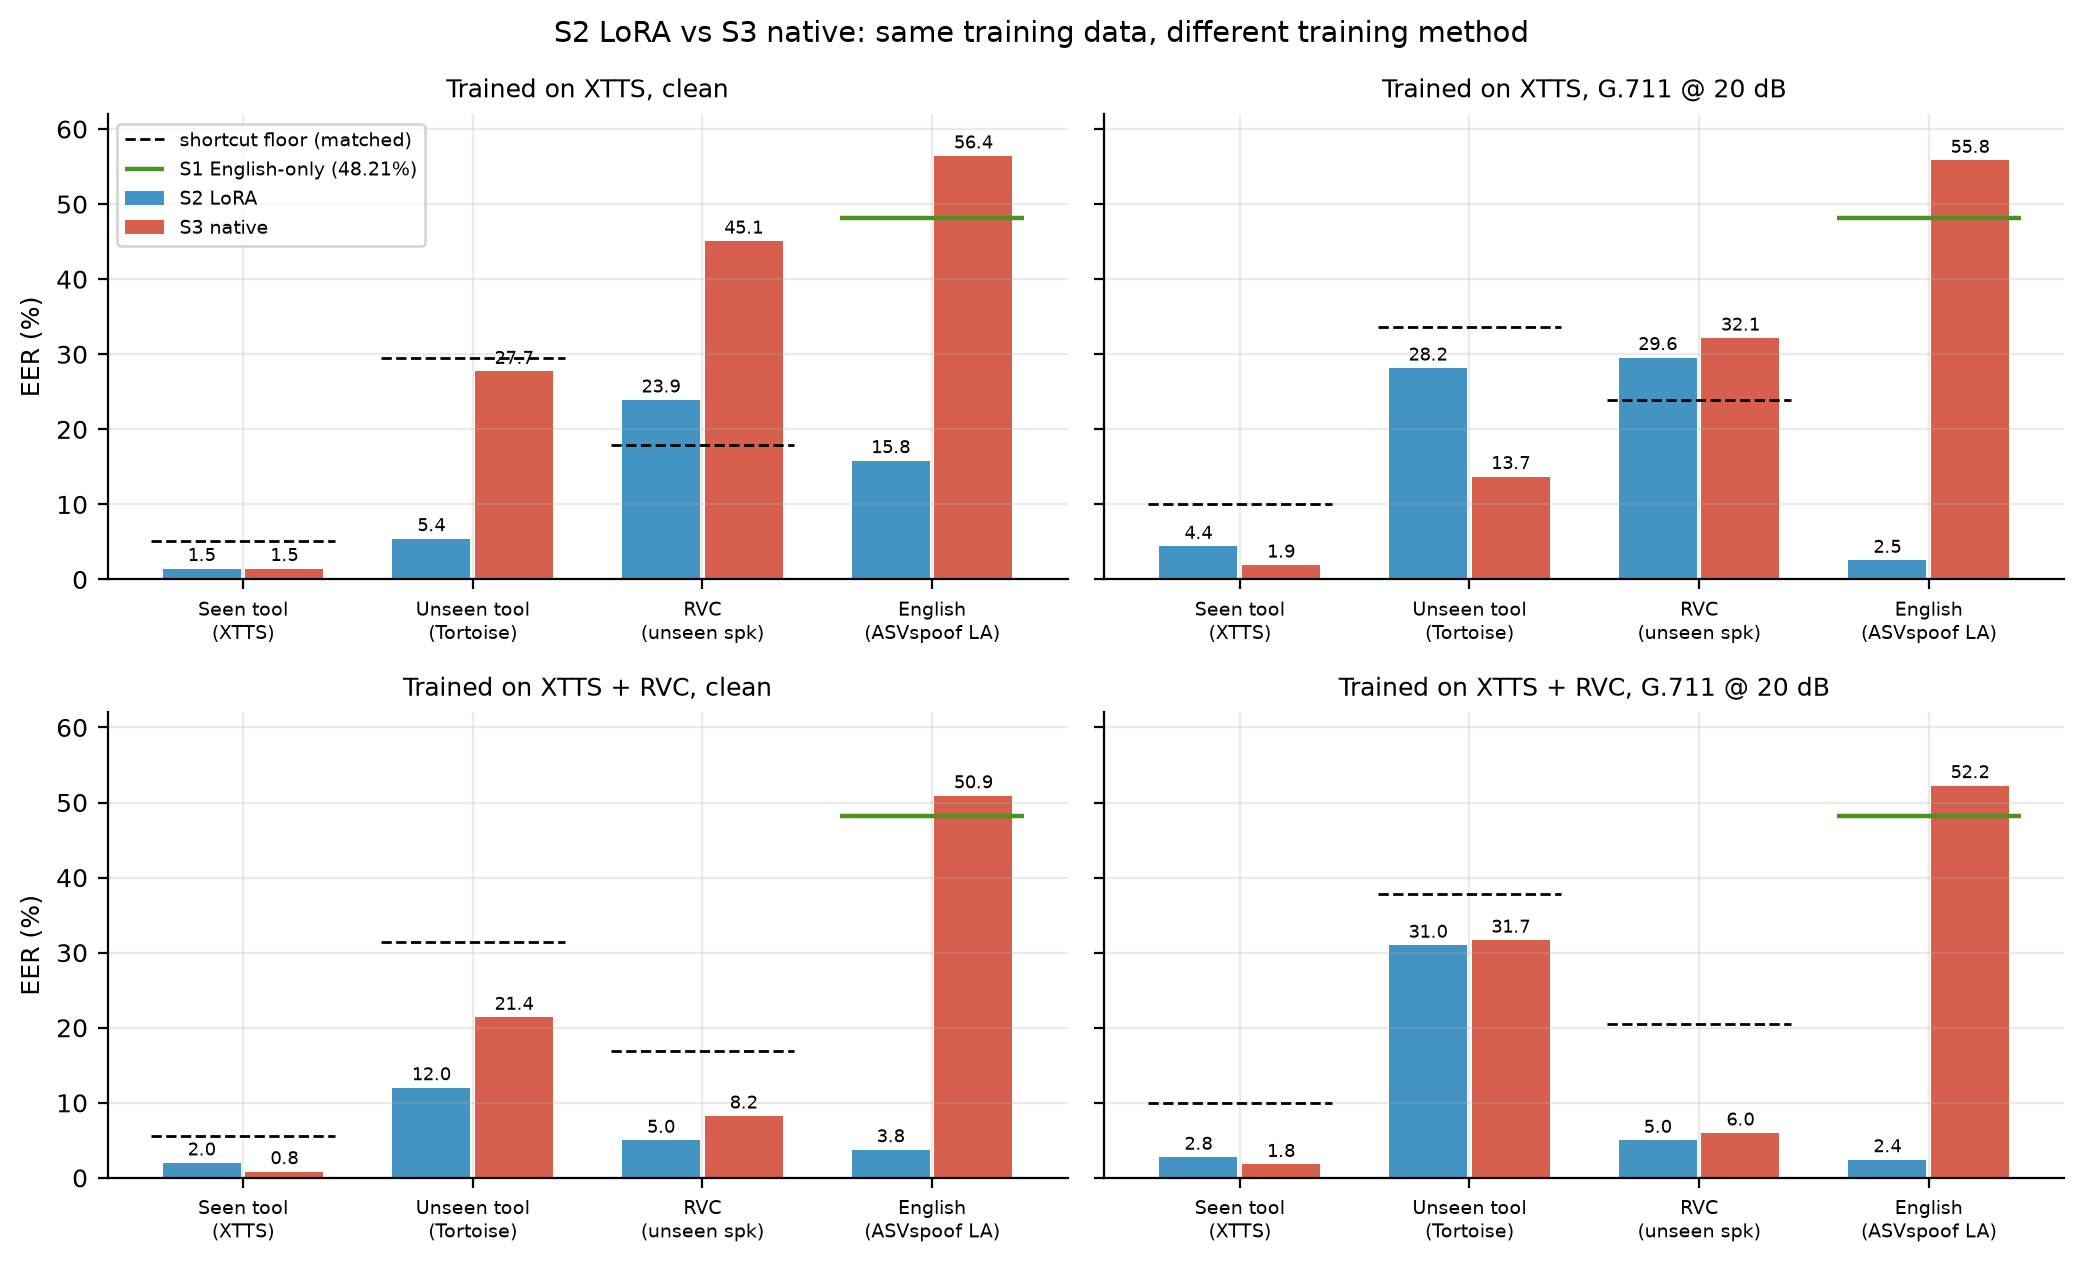
\includegraphics[width=\textwidth]{figures/systems_s2_s3.png}
\caption{S2 (LoRA) and S3 (native) trained on the same data, per training variant.
Dashed lines are matched shortcut floors; the green line is S1 on English.}
\label{fig:systems}
\end{figure*}

Five findings follow.

\textbf{1. A 1\% adapter closes the gap on the seen tool.} Three of the four S2
models beat their evaluation-pool floor at the speaker level: 1.46\% and 1.99\% clean,
and 2.75\% over the telephone channel for the deployed model, 7.21 points under its
floor [$-$12.92, $-$1.10]. The fourth, the XTTS-only channel adapter, scores 4.41\%
against a 10.01\% floor, but with 15 test speakers the paired interval
[$-$12.14, +4.05] reaches zero. Moving 1.13\% of the weights takes the detector from
chance to below the floor on unseen speakers. Retrained with five seeds, the deployed
adapter beats this floor in three and is inconclusive in the other two
(Sec.~\ref{sec:seeds}).

\textbf{2. The adapter must be trained on the deployment channel.} Before
normalisation, an adapter trained on clean audio and scored on channel-rendered
audio rose from 1.34\% to 38.58\% EER, passing most clones as genuine; its cue lay
above 4~kHz, which a narrowband codec removes. Training on channel-rendered audio
recovered 3.89\%. After normalisation, both channel-matched S2 models sit below their
channel floors, the deployed one significantly so (Finding~1). We therefore train and
score each model in the condition it will be used in.
% pre-normalisation figures: docs/results/channel_matched_v1.md

\textbf{3. Attack diversity is not free.} Adding RVC conversions to S2's training
data cuts RVC EER from 23.91\% to 5.01\% clean and from 29.56\% to 5.01\% over the
channel, on speakers unseen as source or target. It also raises EER on the unseen
Tortoise attack, from 5.44\% to 12.01\% clean and from 28.16\% to 30.99\% over the
channel (Fig.~\ref{fig:ablation}); averaged over five training seeds the channel
figures are 25.59\% and 35.59\% (Sec.~\ref{sec:seeds}). Covering one attack family
moved the decision boundary away from another.

\begin{figure}[t]
\centering
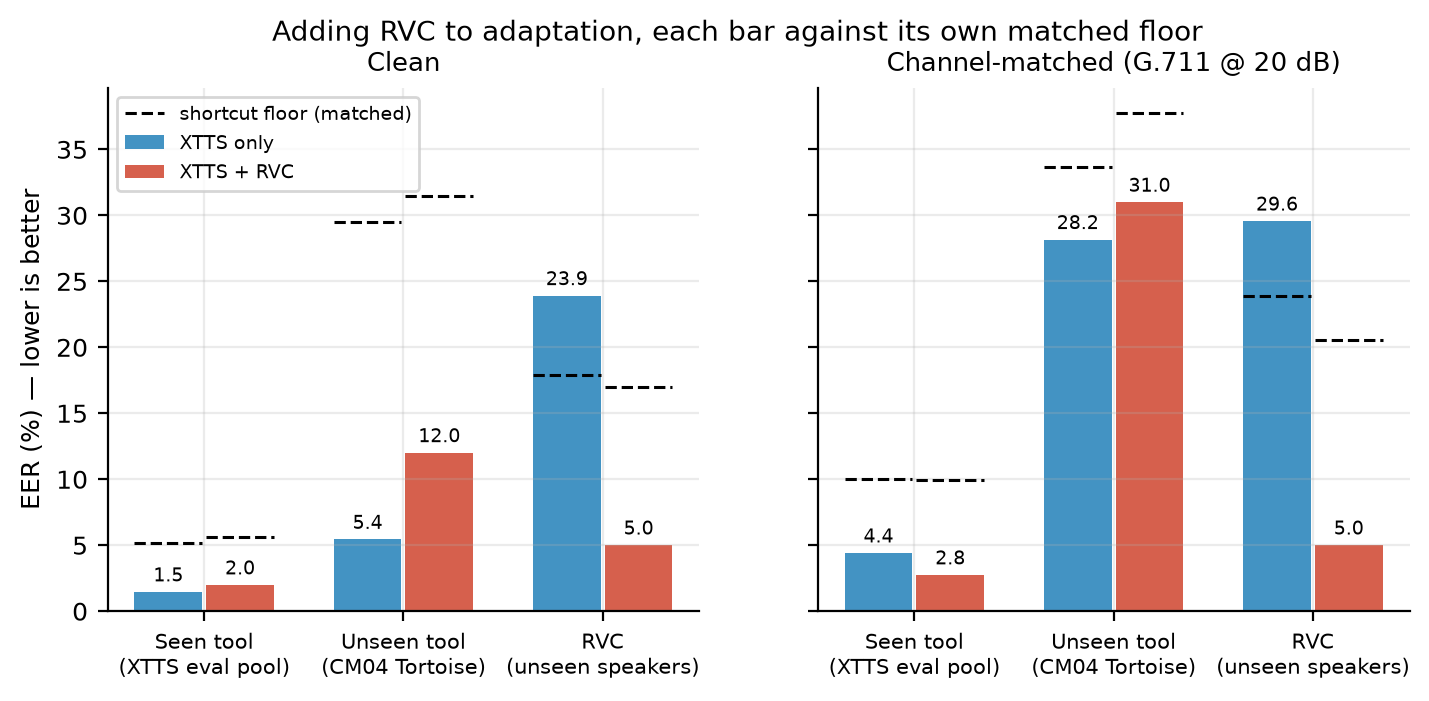
\includegraphics[width=\columnwidth]{figures/ablation_rvc.png}
\caption{Adding RVC to S2's adaptation data, clean and channel-matched. Dashed
lines: the matched shortcut floor of each bar's training data; whether a bar is
evidence is decided by the paired test of Table~\ref{tab:main}.}
\label{fig:ablation}
\end{figure}

\textbf{4. Native training wins on its own data and loses English.} S3 is the most
accurate model on the seen tool, reaching 0.83\% clean with XTTS and RVC in training
against 1.99\% for the matching S2. On English it sits at 50.90--56.42\% EER, which
is chance, in every variant. S2 keeps English at 2.42--3.75\% in three of four
variants; the clean XTTS-only adapter is the exception at 15.83\%. The collapse is
the English-to-code-mixed gap of Sec.~\ref{sec:gap} run in reverse: each model
learns its own training domain's notion of genuine speech. Adaptation keeps S1's
notion and extends it, which is why S2, not S3, is the system we deploy.

\textbf{5. The unseen tool over a telephone line is the weakest result.} On clean
audio both S2 models beat their matched Tortoise floors, 5.44\% and 12.01\% against
29.49\% and 31.43\%. Over the channel one model does: S3 trained on XTTS alone, at
13.71\% against 33.64\%, a paired difference of $-$19.93 points [$-$32.95, $-$8.91];
retrained with five seeds it stays below that floor in all five (mean 19.72\%),
significantly in three. The deployed model reaches 30.99\% in the published run, 6.80
points under its matched floor of 37.79\%, but the speaker interval
[$-$22.32, +8.74] contains zero: it is not shown to lose to the shortcut, and not
shown to beat it. Over five seeds its mean is 35.59\%, and no seed beats the floor;
the published run was a favourable draw. Its error also varies widely by speaker, from
6.4\% to 45.5\% across the 15 test speakers. Adding RVC to channel training is what
removes the Tortoise advantage, for S2 and S3 alike. Detecting a synthesis tool never
seen in training, after a narrowband channel has removed the high frequencies,
remains open, and we report it as the main limitation of this work.

\subsection{Stability across training seeds}
\label{sec:seeds}

Every number above comes from one training run with seed 1234, and the clip-level
intervals of Table~\ref{tab:main} say nothing about training randomness. We therefore
retrained the three phone-line systems that carry the claims of this section with
four further seeds each, the published configurations otherwise unchanged. The
deployed model's seed 1234 was retrained too, and reproduces the published run (CM04
30.14\% against 30.99\%). Table~\ref{tab:seeds} gives the spread across seeds and,
for each seed, the paired speaker-level comparison with the matched floor.

\begin{table*}[t]
\centering
\caption{Five training seeds per system, phone-line condition. EER (\%): mean
$\pm$ standard deviation across seeds, 95\% $t$-interval of the mean, and range. Last
column: seeds whose paired, speaker-level difference from the matched floor lies
wholly below zero, with the floor in brackets.}
\label{tab:seeds}
\small
\begin{tabular}{@{}llcccc@{}}
\toprule
System & Test set & Mean $\pm$ sd & 95\% CI of mean & Range & Seeds beating floor \\
\midrule
S2 XTTS + RVC (deployed) & Eval pool (XTTS) & 3.27 $\pm$ 1.17 & [1.82, 4.73] & 2.42--5.24 & 3 of 5 (9.96) \\
                         & CM04 (Tortoise) & 35.59 $\pm$ 3.35 & [31.43, 39.75] & 30.14--38.43 & 0 of 5 (37.79) \\
                         & RVC test & 5.33 $\pm$ 1.27 & [3.75, 6.91] & 3.71--7.27 & 5 of 5 (20.52) \\
\midrule
S2 XTTS & Eval pool (XTTS) & 3.45 $\pm$ 0.72 & [2.56, 4.34] & 2.75--4.41 & 0 of 5 (10.01) \\
        & CM04 (Tortoise) & 25.59 $\pm$ 5.27 & [19.05, 32.13] & 17.89--30.61 & 1 of 5 (33.64) \\
        & RVC test & 27.07 $\pm$ 2.76 & [23.65, 30.50] & 24.23--30.21 & 0 of 5 (23.91) \\
\midrule
S3 XTTS & Eval pool (XTTS) & 1.78 $\pm$ 0.93 & [0.62, 2.93] & 0.63--3.20 & 4 of 5 (10.01) \\
        & CM04 (Tortoise) & 19.72 $\pm$ 5.36 & [13.06, 26.38] & 13.71--27.07 & 3 of 5 (33.64) \\
        & RVC test & 36.83 $\pm$ 3.39 & [32.62, 41.05] & 32.15--40.39 & 0 of 5 (23.91) \\
\bottomrule
\end{tabular}
\end{table*}

Three points follow. The deployed model is stable where it works: on RVC its standard
deviation across seeds is 1.27 points and it beats its floor in every seed. On the
unseen tool it is not: across seeds it sits two points under its floor, and the
published 30.99\% was close to the best of five runs. S3 trained on XTTS alone is the
more dependable unseen-tool result, below its floor in every seed, at the cost of
RVC, where four of its five seeds are worse than the floor. And the standard
deviation across seeds on CM04 is three to five points for every system, so a
single-run difference of that size between two systems is not evidence.
% src/reporting/seeds.py; experiments/results/seeds_v1.json;
% docs/results/seed_stability_v1.md

\subsection{Changes aimed at the unseen tool}
\label{sec:variants}

We tried three changes to the deployed recipe, each switched on without altering
anything else. The first draws a fresh random crop of every clip in every epoch; the
published recipe reused one crop throughout. The second randomises, on every
training clip, the recording cues the shortcut floor relies on: level ($\pm$6~dB),
spectral tilt ($\pm$3~dB per octave) and coloured noise (10--40~dB SNR), plus a
second G.711 pass at a random 5--30~dB SNR. The third replaces the last encoder layer
with a learned weighting of all of them, since the decision forms by layer~3
(Sec.~\ref{sec:probe}). The rule for choosing was fixed before any run: the lowest
dev EER wins, dev EERs within half a point tie, and a tie goes to the candidate with
fewer changes. The test sets were scored for every candidate but not consulted.

\begin{table}[t]
\centering
\caption{The deployed recipe and its variants, seed 1234, phone-line condition. EER
(\%). The candidate is chosen on dev EER alone.}
\label{tab:variants}
\small
\begin{tabular}{@{}lcccc@{}}
\toprule
Candidate & Dev & Eval pool & CM04 & RVC \\
\midrule
Published recipe (chosen)     & 5.50 & 2.57 & 30.14 & 5.33 \\
+ crop                        & 9.10 & 4.59 & 32.58 & 6.62 \\
+ crop + augment              & 5.34 & 3.38 & 29.49 & 7.59 \\
+ crop + layer mix            & 9.10 & 3.38 & 30.78 & 7.92 \\
+ crop + augment + layer mix  & 9.10 & 3.38 & 26.43 & 7.27 \\
\bottomrule
\end{tabular}
\end{table}

Under the rule the published recipe stays (Table~\ref{tab:variants}). Crop with
augmentation is lowest on dev, at 5.34\%, but within half a point of the recipe's
5.50\%, and the two layer-mix variants are worse on dev. None of the changes improves
the deployed model on its own validation data.

\textbf{An exploratory result.} One variant, crop with augmentation and the layer
mix, had the lowest single-run Tortoise error (26.43\%), below every seed of the
published recipe. Because it was singled out after a test score had been seen, what
follows is exploratory. Retrained with four further seeds, it averages 26.63\%
$\pm$ 1.66 on Tortoise against 35.59\% $\pm$ 3.35 for the published recipe, and all
five of its seeds fall below all five of the recipe's (exact Mann--Whitney
$p = 0.008$; $p = 0.016$ on the four seeds trained after the choice). The gain has a
price: RVC rises from 5.33\% to 7.72\% ($p = 0.03$), still below its floor in every
seed. Against the Tortoise floor the variant remains inconclusive in every seed, at
$-$9.0 to $-$13.6 points with speaker intervals that reach zero. Its dev EER is no
better than the recipe's (7.11\% against 6.96\%, averaged over seeds): the in-domain
dev set does not see unseen-tool generalisation, so a rule that selects on it cannot
find this kind of improvement. We report the variant as a lead to be confirmed on a
second unseen tool, not as a validated result.
% src/reporting/variants.py; experiments/results/variants_v1.json;
% docs/results/variants_v1.md

\subsection{New speakers and a second unseen tool}
\label{sec:res-new}

The original test pool has 15 speakers and one unseen tool. Section~\ref{sec:data-extension}
adds 60 speakers no model has heard, cloned with the seen tool (CM05) and with Tortoise
(CM06), and a second unseen generator, IndicF5 (CM07), on 54 test speakers.
Table~\ref{tab:new} scores every system in its own training condition.

\begin{table}[t]
\centering
\caption{EER (\%) on the week-13 sets, each system in its training condition; 95\%
speaker-bootstrap intervals. New speakers: 60 speakers, 2{,}400 genuine clips.
IndicF5: clones of 54 speakers, 651 all-Hindi genuine clips of 75.}
\label{tab:new}
\small
\begin{tabular}{@{}lrrr@{}}
\toprule
System, audio & XTTS (seen) & Tortoise & IndicF5 \\
\midrule
S1, channel & 44.8 {\scriptsize[40.8, 48.8]} & 52.7 {\scriptsize[48.7, 57.8]} & 51.3 {\scriptsize[46.1, 56.5]} \\
S2 XTTS, clean & 7.2 {\scriptsize[4.3, 10.0]} & 13.5 {\scriptsize[10.4, 17.5]} & 37.0 {\scriptsize[33.9, 41.4]} \\
S2 XTTS, channel & 7.4 {\scriptsize[5.5, 9.5]} & 29.7 {\scriptsize[25.6, 33.2]} & 43.9 {\scriptsize[39.9, 47.9]} \\
S2 XTTS+RVC, clean & 10.2 {\scriptsize[5.9, 14.1]} & 26.1 {\scriptsize[21.4, 30.0]} & 34.4 {\scriptsize[30.1, 38.6]} \\
Deployed S2, channel & 9.4 {\scriptsize[6.6, 12.5]} & 29.4 {\scriptsize[25.4, 33.3]} & 30.6 {\scriptsize[26.7, 34.9]} \\
\bottomrule
\end{tabular}
% docs/results/new_speakers_v1.md; experiments/results/ext_scoring_v1/
\end{table}

\textbf{The seen tool transfers to new people.} Over the channel the deployed model
reaches 9.4\% EER on 60 new speakers, against 2.75\% on the original 15; the median
speaker sits at 2.9\% and the worst at 17.1\%, so the rise comes from a wider spread of
voices rather than from a few speakers failing. S1 stays at 44.8\%.

\textbf{Both unseen tools stay hard over the channel.} Tortoise on the new speakers
lands where it did on the original pool: 29.4\% for the deployed model and 29.7\% for
the XTTS-only channel adapter. IndicF5, a newer generator, is no easier, at 30.6\%
for the deployed model, which is the best system on it; the clean adapters reach
34.4--37.0\% on clean IndicF5. On clean audio the XTTS-only adapter generalises to
Tortoise on new speakers as it did on the original ones (13.5\%), but not to IndicF5
(37.0\%). One unseen tool can be generalised to on clean audio; neither survives the
telephone channel, and the two unseen tools behave alike over it.

\textbf{Against the matched floors.} With each system's floor fitted on its own
training data and paired clip by clip (\texttt{docs/results/floor\_new\_sets\_v1.md}),
every S2 system is below its floor on the new speakers for both XTTS and Tortoise; the
deployed model by 28.6 [$-$33.1, $-$24.5] and 28.8 [$-$33.9, $-$23.8] points. That
result is weaker than it looks: the Tortoise floors land at 40--58\%, near or past
chance, because the recording cues that separate the training clips do not carry to
the new speakers' recordings. On IndicF5 the floors stay informative (34.0--35.9\%)
and no system clears one: the deployed model is inconclusive ($-$5.4 [$-$11.2, +1.5]),
the clean adapters are level with theirs, and the XTTS-only channel adapter is worse
than its floor (+9.9 [+3.3, +16.5]). The second unseen tool therefore confirms the
paper's weakest result rather than relieving it.

\textbf{A real mobile codec undoes much of the channel training.} Passing the same sets
through the reference AMR-NB codec at 12.2~kbit/s instead of the simulated G.711 line,
the deployed model rises from 9.4\% to 23.7\% {\scriptsize[19.6, 27.4]} on new-speaker
XTTS, from 29.4\% to 37.0\% on Tortoise, from 30.6\% to 47.0\% on IndicF5, and to
40.6\% on CM04. The clean-trained adapter holds better on AMR-NB (12.6\% on XTTS) than
the channel-trained one, because AMR-NB keeps the voice band and adds no noise, so it
sounds closer to clean audio than to the noisy G.711 render. Training over the channel
taught the deployed model one telephone chain, not telephone audio in general; a service
on mobile networks needs real codecs in training (\texttt{docs/results/amr\_channel\_v1.md}).

Training on both does it. The deployed recipe trained on every clip over G.711 and again
through AMR-NB, three seeds against the deployed recipe, is better on AMR-NB in every seed:
new-speaker XTTS 7.59\% against 22.37\%, Tortoise 19.52\% against 36.48\%, IndicF5
28.01\% against 46.13\% and CM04 14.92\% against 36.76\%, while over G.711 it is level
or better (IndicF5 27.10\% against 31.24\%; \texttt{experiments/results/mixcodec\_v1/}).
Three seeds cannot reach significance (the smallest exact two-sided $p$ is 0.25 paired,
0.10 unpaired), but the gaps are four to twenty standard deviations wide.

\subsection{More genuine speakers}
\label{sec:res-speakers}

The deployed S2 adapts on 21 genuine speakers. We retrained the same recipe, changing
only the training manifest, on 248: the 227 extra adaptation speakers
(Section~\ref{sec:data-extension}) and their CM08 clones. Both recipes were trained with
the same five seeds and scored on every set over the channel (Table~\ref{tab:speakers248}).
Here, as in Sec.~\ref{sec:res-final}, the deployed recipe is retrained in the same run as the
recipe it is compared with, so its numbers differ a little from table to table (CM04 over the
channel: 35.59\% in Table~\ref{tab:seeds}, 33.46\% here, 36.2\% in Table~\ref{tab:final}),
always within the seed-to-seed spread; every comparison is made within one run.

\begin{table}[t]
\centering
\caption{The deployed recipe trained on 21 against 248 genuine speakers: EER (\%) and
false alarms over the channel, mean $\pm$ sd over five seeds. Every seed of the
248-speaker recipe beats every seed of the 21-speaker recipe on each starred row
(exact Mann--Whitney $p = 0.008$, the smallest possible for five against five).}
\label{tab:speakers248}
\small
\begin{tabular}{@{}lrr@{}}
\toprule
Set & 21 speakers & 248 speakers \\
\midrule
New speakers, XTTS$^*$       & 10.75 $\pm$ 0.94 & \textbf{0.91} $\pm$ 0.33 \\
New speakers, Tortoise$^*$   & 29.82 $\pm$ 1.73 & \textbf{13.59} $\pm$ 3.39 \\
CM04 Tortoise$^*$            & 33.46 $\pm$ 2.63 & \textbf{24.48} $\pm$ 3.48 \\
IndicF5$^*$                  & 35.40 $\pm$ 1.64 & \textbf{27.25} $\pm$ 0.68 \\
Original test pool$^*$       & 3.42 $\pm$ 0.44  & \textbf{1.12} $\pm$ 0.31 \\
RVC test half                & 5.78 $\pm$ 0.67  & 6.49 $\pm$ 1.88 \\
False alarms, control$^*$    & 3.40 $\pm$ 1.60  & \textbf{0.47} $\pm$ 0.38 \\
\bottomrule
\end{tabular}
% docs/results/w13_runs_v1.md; experiments/results/overfit_fix_v1/
\end{table}

\textbf{Voices, not attacks, were the bottleneck.} Hearing 248 genuine speakers instead
of 21 improves six of seven sets in every seed. The seen tool on new people falls from
10.75\% to 0.91\%, so the earlier rise on new speakers was the model having heard too
few voices. The unseen tools improve as much: Tortoise on the new speakers from 29.82\%
to 13.59\%, CM04 from 33.46\% to 24.48\%, IndicF5 from 35.40\% to 27.25\%, and genuine
callers are called fake seven times less often (0.47\% against 3.40\%). Only RVC, whose
training conversions are unchanged, stays level. The added data are genuine speech and
clones by the \emph{seen} tool only; no Tortoise or IndicF5 audio entered training, so
the unseen-tool gains come from a broader notion of genuine speech, not from exposure to
the attacks.

\textbf{Spontaneous speech does not improve.} The added speakers read lectures, like the
original ones. On the 24 spontaneous HiACC speakers, the seed-1234 model trained on 248
speakers falsely flags 46.0\% [38.8, 53.3] of genuine clips over the channel, against
38.5\% [28.2, 48.7] for the deployed recipe retrained in the same run: the intervals
overlap and the point estimate is not better. (The published deployed checkpoint scored
54.4\%, so two trainings of one recipe differ by that much; one seed each here.) More
read voices do not teach the detector what spontaneous speech sounds like, and neither
does the real codec: the final recipe's seed-1234 model calls 43.9\% [36.5, 51.2] of the
same clips fake. That is 10.5 points below the published deployed checkpoint on identical
clips (paired speaker bootstrap $[-17.1, -3.8]$; 16 of 24 speakers lower), but it lies
inside the 38.5--54.4\% spread of single trainings, so with one seed it is not evidence
that the recipe helps. Spontaneous speech needs spontaneous training data, which the
dataset rules keep HiACC from supplying
(\texttt{docs/results/hiacc\_final\_v1.md}).

\subsection{The final recipe}
\label{sec:res-final}

The two largest gains so far came separately: more genuine speakers
(Sec.~\ref{sec:data-extension}) and real AMR-NB audio in training next to the simulated
G.711 line. The final recipe uses both: the adapter is trained on the 248-speaker set,
every clip in both codecs (16{,}036 clips), with the same dev set and the same five seeds
as the deployed adapter (Table~\ref{tab:final}).

\begin{table}[t]
\centering
\caption{The final recipe against the deployed adapter (21 speakers, G.711 only): EER
(\%) mean $\pm$ sd over five paired seeds; last line, genuine clips called fake. The final
recipe is better in every seed except on RVC (worse in all five) and false alarms (better
in four of five).}
\label{tab:final}
\footnotesize
\setlength{\tabcolsep}{3pt}
\begin{tabular}{@{}lrr@{}}
\toprule
Test set (phone line) & Final & Deployed \\
\midrule
Original test pool & 1.1 $\pm$ 0.2 & 3.5 $\pm$ 0.8 \\
New speakers, XTTS (seen tool) & 0.9 $\pm$ 0.3 & 12.0 $\pm$ 1.9 \\
New speakers, Tortoise & 8.8 $\pm$ 1.4 & 30.8 $\pm$ 2.1 \\
CM04, Tortoise & 17.7 $\pm$ 2.3 & 36.2 $\pm$ 5.5 \\
CM07, IndicF5 & 21.7 $\pm$ 3.7 & 34.9 $\pm$ 1.4 \\
RVC test half (worse in all five) & 8.5 $\pm$ 1.9 & 6.1 $\pm$ 0.7 \\
Genuine called fake & 0.5 $\pm$ 0.7 & 2.4 $\pm$ 1.2 \\
\midrule
\multicolumn{3}{@{}l}{\emph{Real AMR-NB codec}} \\
New speakers, XTTS & 0.7 $\pm$ 0.2 & 23.2 $\pm$ 0.9 \\
New speakers, Tortoise & 6.0 $\pm$ 1.2 & 36.3 $\pm$ 2.3 \\
CM04, Tortoise & 6.9 $\pm$ 2.1 & 37.9 $\pm$ 3.8 \\
CM07, IndicF5 & 21.3 $\pm$ 2.3 & 46.5 $\pm$ 1.2 \\
\bottomrule
\end{tabular}
% docs/results/final_recipe_v1.md; experiments/results/final_v1/
\end{table}

\textbf{Better on ten of eleven sets, in every seed on nine of them.} Over the simulated line the new
speakers' seen tool falls from 12.0\% to 0.9\%, new-speaker Tortoise from 30.8\% to 8.8\%
and CM04 from 36.2\% to 17.7\%; over the real AMR-NB codec, where the deployed adapter is
near chance (36--47\% on the unseen tools), the final recipe reaches 6.0--6.9\% on both
Tortoise sets. No unseen-tool audio entered training.

\textbf{RVC is the exception.} Error on the voice-conversion half rises from 6.1\% to
8.5\%, in all five seeds. We have not isolated the cause. The added speakers have XTTS
clones but no RVC conversions, so the share of conversion audio falls, which may explain
it. We report it as a cost of the larger set.

\textbf{Against its shortcut floor.} Both systems trained on the final data share one
floor: the eight statistics fitted on the final training set and scored on each detector's
own clips, with the speaker-level paired test of Sec.~\ref{sec:floors}. Every one of
the five adapter seeds beats it on all eleven sets. On the unseen tools the floor is
informative and the margin is wide: new-speaker Tortoise 8.8\% against a floor of 36.5\%,
IndicF5 21.7\% against 38.8\% (21.3\% against 37.8\% over AMR-NB). The deployed recipe
beat its Tortoise floor over the channel in no seed. On three sets, CM04 over either codec
and new-speaker Tortoise over AMR-NB, the floor is above chance (54.6--71.4\%): the cheap
statistics rank genuine and fake the wrong way round on those recordings, so beating it
there shows only that the detector does not lean on those cues
(\texttt{docs/results/floor\_final\_v1.md}).

\textbf{What we have not shown.} With five paired seeds the smallest possible exact $p$ is
$0.0625$ per set, so the comparison with the deployed recipe rests on the direction being
the same in every seed. IndicF5 (21.7\%) and, below, Chatterbox stay hard.

\subsection{A third unseen tool}
\label{sec:res-chatterbox}

Chatterbox (CM09) is a third generator family none of our training data resembles: XTTS-v2
is an autoregressive decoder, Tortoise adds diffusion, IndicF5 uses flow matching, and
Chatterbox is a recent multilingual cloner. We scored the same models on its 525 clips
against the same 651 genuine all-Hindi clips as IndicF5 (Table~\ref{tab:chatterbox}).

\begin{table}[t]
\centering
\caption{EER (\%) on Chatterbox (CM09) with 95\% bootstrap intervals. The 248-speaker
adapter is trained over both telephone codecs and is one seed (1234); the others are the
models of the earlier tables.}
\label{tab:chatterbox}
\footnotesize
\begin{tabular}{@{}lrr@{}}
\toprule
Detector & Phone line & Clean \\
\midrule
S1, English only             & 55.0 [52.9, 57.7] & 61.1 [58.7, 63.9] \\
Adapter, 21 speakers         & 35.8 [33.4, 38.8] & 48.0 [44.9, 50.3] \\
Adapter, 248 speakers, 2 codecs & 32.0 [30.0, 34.9] & 49.0 [45.8, 52.2] \\
\bottomrule
\end{tabular}
% experiments/results/cm09_v1/
\end{table}

\textbf{It is the hardest unseen tool.} The best detector reaches 32.0\% over the phone
line, against 9.0\% for the same model (seed 1234) on new-speaker Tortoise and 25.7\% on IndicF5, and
clean audio is near chance for both adapters (48--49\%). The English-only S1 is at 55.0\%.

\textbf{The added voices help little here.} The 248-speaker adapter is 3.8 points better
than the 21-speaker one over the phone line (the intervals overlap, and it is one seed), far
less than the 11 to 22 points it gained on XTTS and Tortoise. Training on more genuine
speakers closed the gap for tools that resemble the training clones; it did not carry over
to a generator of a different family.

\textbf{The watermark did not help.} Chatterbox marks its output, yet no detector found
it: the scores are worse than for IndicF5, so the watermark does not appear to be a
shortcut they use. We report this as a limit: a tool we did not train on can still defeat the detector,
and we have not tried to detect the watermark itself.

\subsection{An outside baseline}
\label{sec:res-aasist}

To place our detector against an established one, we scored AASIST~\cite{jung2022aasist},
a widely used end-to-end anti-spoofing network, with its published weights
(trained on ASVspoof 2019 LA) and then fine-tuned it on exactly the training sets of
Table~\ref{tab:speakers248} with the same dev set (up to 15 epochs, best dev epoch kept;
Table~\ref{tab:aasist}).

\begin{table*}[t]
\centering
\caption{AASIST against our LoRA adapter on the same training data, over the channel:
EER (\%) mean $\pm$ sd over seeds (false alarms in the last column). AASIST: 4 seeds on 21
speakers, 3 on 248; adapter: 5 seeds each. Zero-shot is the published checkpoint.}
\label{tab:aasist}
\footnotesize
\setlength{\tabcolsep}{3pt}
\begin{tabular}{@{}lrrrrrr@{}}
\toprule
System & New XTTS & New Tort. & CM04 & IndicF5 & RVC & False al. \\
\midrule
AASIST, zero-shot     & 46.3 & 54.1 & 52.4 & 54.7 & 46.7 & 82.3 \\
\midrule
AASIST, 21 speakers   & 14.1 $\pm$ 1.1 & 26.9 $\pm$ 1.1 & 29.5 $\pm$ 6.7 & 27.1 $\pm$ 1.2 & 6.7 $\pm$ 0.7 & 19.0 $\pm$ 18.9 \\
Adapter, 21 speakers  & 10.8 $\pm$ 0.9 & 29.8 $\pm$ 1.7 & 33.5 $\pm$ 2.6 & 35.4 $\pm$ 1.6 & 5.8 $\pm$ 0.7 & 3.4 $\pm$ 1.6 \\
\midrule
AASIST, 248 speakers  & 1.8 $\pm$ 0.3 & \textbf{9.6} $\pm$ 1.6 & \textbf{16.7} $\pm$ 0.5 & 26.4 $\pm$ 1.6 & 13.5 $\pm$ 0.4 & 2.3 $\pm$ 0.8 \\
Adapter, 248 speakers & \textbf{0.9} $\pm$ 0.3 & 13.6 $\pm$ 3.4 & 24.5 $\pm$ 3.5 & 27.3 $\pm$ 0.7 & \textbf{6.5} $\pm$ 1.9 & \textbf{0.5} $\pm$ 0.4 \\
\bottomrule
\end{tabular}
% docs/results/w13_runs_v1.md; experiments/results/aasist_v1/
\end{table*}

\textbf{An English detector fails the same way.} Zero-shot, AASIST rejects 82.3\% of
genuine Hindi--English speech and sits at 43--55\% EER on every attack set, the failure
of our English-trained S1: the gap is not particular to one architecture.

\textbf{After fine-tuning, neither system wins everywhere.} On the 248 speakers, AASIST
is better on the two unseen Tortoise sets (CM04 16.7\% against 24.5\%, exact
Mann--Whitney $p = 0.036$, the smallest possible for three against five seeds; new
speakers 9.6\% against 13.6\%, $p = 0.14$) and level on IndicF5. The LoRA adapter is better on the
seen tool (0.9\% against 1.8\%), on RVC (6.5\% against 13.5\%, $p = 0.036$) and in false
alarms (0.5\% against 2.3\%, $p = 0.036$). With 21 speakers AASIST is also unstable: its
false alarms range up to 47\% for one seed. Both systems gain far more from the
248 speakers than they differ from each other, for example AASIST on new-speaker
Tortoise falls from 26.9\% to 9.6\%. The voices matter more than the architecture.
These are the first fine-tunings of AASIST on this data with a recipe tuned for neither
system, and with fewer seeds than the adapter, so the comparison is indicative.

\subsection{A stronger outside baseline}
\label{sec:res-sslaasist}

AASIST uses a small convolutional front end. The closest outside system to ours is
SSL-AASIST~\cite{tak2022wav2vec}, the same back end on a wav2vec 2.0 XLS-R 300M encoder,
which has about three times the parameters of our wav2vec2-base encoder. We ported it to
Hugging Face (it loads the published checkpoint and scores 0.0\% EER on ASVspoof clips in
our checks), scored the published weights, and fine-tuned the whole network on the same two
training sets as the adapter, with RawBoost and the dev epoch kept (Table~\ref{tab:sslaasist}).

\begin{table*}[t]
\centering
\caption{SSL-AASIST against our LoRA adapter on the same G.711 training data: EER (\%)
mean $\pm$ sd over seeds, false alarms in the last column. SSL-AASIST: 3 seeds on 21
speakers, 2 on 248; adapter: 5 seeds each.}
\label{tab:sslaasist}
\footnotesize
\setlength{\tabcolsep}{3pt}
\begin{tabular}{@{}lrrrrrr@{}}
\toprule
System & New XTTS & New Tort. & CM04 & IndicF5 & RVC & False al. \\
\midrule
SSL-AASIST, zero-shot & 22.7 & 32.9 & 29.1 & 53.0 & 44.1 & 73.1 \\
\midrule
SSL-AASIST, 21 spk. & 2.1 $\pm$ 1.0 & 7.8 $\pm$ 1.3 & 5.0 $\pm$ 2.7 & 24.1 $\pm$ 1.8 & 2.6 $\pm$ 1.2 & 3.7 $\pm$ 2.2 \\
Adapter, 21 spk. & 10.8 $\pm$ 0.9 & 29.8 $\pm$ 1.7 & 33.5 $\pm$ 2.6 & 35.4 $\pm$ 1.6 & 5.8 $\pm$ 0.7 & 3.4 $\pm$ 1.6 \\
\midrule
SSL-AASIST, 248 spk. & \textbf{0.1} $\pm$ 0.1 & \textbf{0.5} $\pm$ 0.1 & \textbf{1.1} $\pm$ 0.3 & \textbf{16.5} $\pm$ 1.0 & \textbf{4.9} $\pm$ 0.2 & \textbf{0.2} $\pm$ 0.2 \\
Adapter, 248 spk. & 0.9 $\pm$ 0.3 & 13.6 $\pm$ 3.4 & 24.5 $\pm$ 3.5 & 27.3 $\pm$ 0.7 & 6.5 $\pm$ 1.9 & 0.5 $\pm$ 0.4 \\
\bottomrule
\end{tabular}
% docs/results/ssl_aasist_v1.md; experiments/results/ssl_aasist_v1/
\end{table*}

\textbf{The same failure zero-shot.} The published SSL-AASIST rejects 73.1\% of genuine
Hindi--English speech over the phone line and sits at 22.7--53.0\% EER on the attack sets,
so even a strong English-trained detector shows the gap.

\textbf{A larger encoder is stronger once it sees the voices.} Fine-tuned on the 248
speakers it is lower than our adapter on every set: Tortoise from new speakers 0.5\%
against 13.6\%, CM04 1.1\% against 24.5\%, IndicF5 16.5\% against 27.3\%, and false alarms
0.2\% against 0.5\%. The same holds with 21 speakers. We read this as the encoder, and in
part the full fine-tuning, not the training recipe. The recipe still does what it did for
the adapter: SSL-AASIST on 21 speakers is 24.1\% on IndicF5 and 5.0\% on CM04, and the added
voices cut CM04 to 1.1\%, so the voices help it as much. Two caveats: SSL-AASIST has fewer
seeds (two or three) and this table is over the simulated G.711 line only; the next
subsection adds the real AMR-NB codec and Chatterbox, and the spontaneous HiACC set was not
run, so the comparison is indicative. What it does not
change is the main finding: more genuine speakers, not more attack tools, closes most of the
gap.

\subsection{The larger encoder on the final recipe}
\label{sec:res-finalssl}

The comparison above used the G.711-only training sets. We trained SSL-AASIST on exactly
the data of the final recipe (248 speakers, both telephone codecs, 16{,}036 clips), with the
same recipe as before (whole network, RawBoost, three epochs) and the five seeds of the
adapter (1234, 2025, 7, 42, 99), and scored it on everything the adapter was scored on, plus
Chatterbox (Table~\ref{tab:finalssl}). Fig.~\ref{fig:overview} sets every main system
against every attack tool on both telephone channels.

\begin{figure*}[t]
\centering
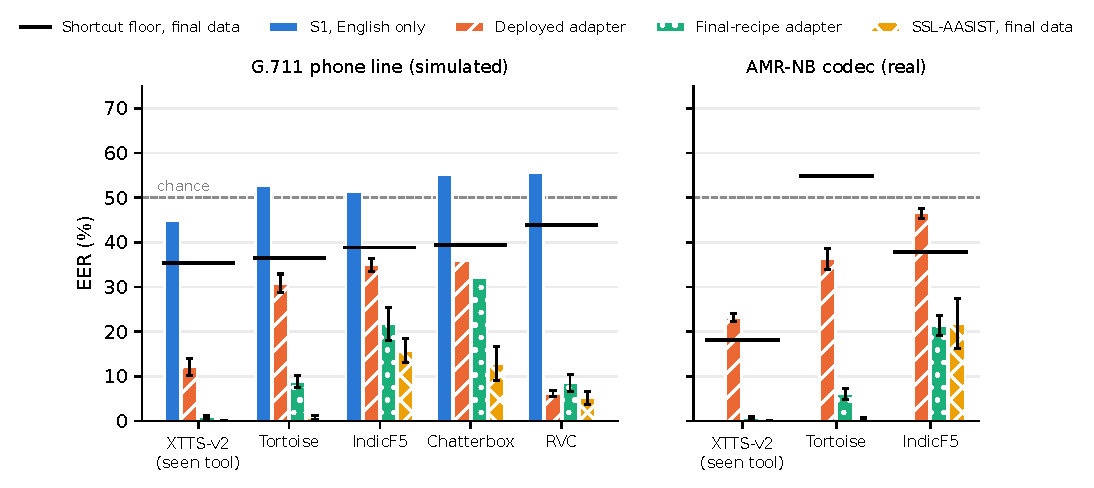
\includegraphics[width=\textwidth]{figures/final_overview.pdf}
\caption{EER of the four main systems on every attack tool, over the simulated G.711 line
(left) and the real AMR-NB codec (right; S1 was not scored there). Bars are means over
five training seeds with one standard deviation; S1 and Chatterbox for both adapters are one
model each. The black tick is the shortcut floor fitted on the final training data, which
belongs to the two final systems; the dashed line is chance. Hatching repeats the colour
for greyscale print.}
\label{fig:overview}
\end{figure*}

\begin{table}[t]
\centering
\caption{SSL-AASIST against the adapter, both trained on the final-recipe data over five
seeds: EER (\%) mean $\pm$ sd, and the exact Mann--Whitney $p$ (smallest possible: 0.008).
AMR-NB is the real mobile codec. Chatterbox: the adapter has one seed.}
\label{tab:finalssl}
\footnotesize
\setlength{\tabcolsep}{3pt}
\begin{tabular}{@{}lrrr@{}}
\toprule
Test set & SSL-AASIST & Adapter & $p$ \\
\midrule
New speakers, XTTS (seen tool) & 0.02 $\pm$ 0.03 & 0.94 $\pm$ 0.34 & 0.008 \\
New speakers, Tortoise & 0.73 $\pm$ 0.38 & 8.81 $\pm$ 1.43 & 0.008 \\
CM04, Tortoise & 1.75 $\pm$ 0.71 & 17.73 $\pm$ 2.27 & 0.008 \\
CM07, IndicF5 & 15.79 $\pm$ 2.61 & 21.68 $\pm$ 3.74 & 0.056 \\
RVC test half & 5.17 $\pm$ 1.51 & 8.53 $\pm$ 1.91 & 0.024 \\
Genuine called fake & 0.29 $\pm$ 0.33 & 0.51 $\pm$ 0.67 & 0.802 \\
Chatterbox (CM09) & 12.86 $\pm$ 3.83 & 31.98 & --- \\
\midrule
\multicolumn{4}{@{}l}{\emph{Real AMR-NB codec}} \\
New speakers, XTTS & 0.05 $\pm$ 0.07 & 0.69 $\pm$ 0.24 & 0.008 \\
New speakers, Tortoise & 0.51 $\pm$ 0.21 & 6.04 $\pm$ 1.17 & 0.008 \\
CM04, Tortoise & 1.36 $\pm$ 0.31 & 6.90 $\pm$ 2.06 & 0.008 \\
CM07, IndicF5 & 21.75 $\pm$ 5.58 & 21.32 $\pm$ 2.27 & 0.690 \\
\bottomrule
\end{tabular}
% docs/results/ssl_vs_adapter_v1.md; experiments/results/final_ssl_v1/, final_ssl_seeds2_v1/
\end{table}

\textbf{Better in every seed on eight of eleven sets.} Over the real AMR-NB codec, error on
new-speaker Tortoise is 0.51\% against 6.04\% for the adapter. On the seen tool, on both
Tortoise sets and on the same sets over AMR-NB, all five SSL-AASIST seeds are below all
five adapter seeds (exact $p = 0.008$); on the RVC half every paired seed is better, with
overlapping ranges ($p = 0.024$). On Chatterbox, the hardest tool, the five seeds range from
8.2\% to 18.3\%, every one below the adapter's single 32.0\%.

\textbf{Level on three.} False alarms (0.29\% against 0.51\%, four seeds of five), IndicF5
over G.711 (15.8\% against 21.7\%, four of five, $p = 0.056$) and IndicF5 over AMR-NB (21.8\%
against 21.3\%) are not separated by five seeds.

\textbf{IndicF5 remains hard for both.} Neither encoder brings it below 15\% on average, and
the larger encoder's seeds range from 13.5\% to 28.1\% over the codec. We have not tested
why; IndicF5's clones are the most natural of the tools we used
(Sec.~\ref{sec:data-extension}), which may make them the hardest.

\textbf{It can run on a live call.} The larger encoder has 316 million parameters against
94 million for wav2vec2-base. One 4\,s window takes 69\,ms on a T4 GPU and 1.14\,s on two
CPU threads (wav2vec2-base: 25\,ms and 0.40\,s). The live path scores a window every 2\,s,
so even on that CPU it keeps up, at 57\% of the budget. Against the same floor as the
adapter, every one of its seeds is below it on every set, Chatterbox included (12.9\%
against 39.5\%).

\textbf{On spontaneous speech it depends on the seed.} Two further trainings (seeds 1234
and 2025) were scored on HiACC's 3{,}318 genuine spontaneous clips. One calls 5.8\%
{\scriptsize[3.2, 9.1]} of them fake, with 5 of 24 speakers above 10\%; the other 46.7\%
{\scriptsize[37.6, 55.7]}, with 23 of 24 above 10\%, where the adapter's final-recipe model
is at 43.9\%. Both reach 0\% EER on the dev set, so nothing in our model selection can tell
them apart. The larger encoder can learn a notion of genuine speech that covers spontaneous
talk, but it does not do so reliably without spontaneous speech in training
(\texttt{docs/results/encoder\_spontaneous\_v1.md}).

\subsection{The deployment trade-off}
\label{sec:tradeoff}

Finding~2 trains each adapter in the condition it will be used in.
Table~\ref{tab:tradeoff} shows what that choice costs: every S2 adapter scored in the
condition it was \emph{not} trained in, to be read against its own row in
Table~\ref{tab:main}.

\begin{table*}[t]
\centering
\caption{S2 adapters scored in the condition they were not trained in. EER (\%) with
95\% bootstrap confidence intervals over clips. The same adapters in their own
condition are in Table~\ref{tab:main}.}
\label{tab:tradeoff}
\small
\begin{tabular}{@{}llccc@{}}
\toprule
Training attacks & Trained $\rightarrow$ scored & Eval pool (XTTS) & CM04 (Tortoise) & RVC test \\
\midrule
XTTS       & clean $\rightarrow$ channel & 27.64 {\scriptsize[26.55, 29.18]} & 18.98 {\scriptsize[16.74, 21.24]} & 39.74 {\scriptsize[36.49, 44.10]} \\
XTTS       & channel $\rightarrow$ clean & 12.51 {\scriptsize[11.70, 13.59]} & 18.78 {\scriptsize[16.50, 20.77]} & 31.50 {\scriptsize[28.11, 35.22]} \\
XTTS + RVC & clean $\rightarrow$ channel & 22.97 {\scriptsize[21.59, 24.36]} & 31.02 {\scriptsize[27.97, 33.70]} & 26.49 {\scriptsize[23.26, 29.72]} \\
XTTS + RVC & channel $\rightarrow$ clean & 6.71 {\scriptsize[6.03, 7.57]}    & 18.33 {\scriptsize[16.23, 20.59]} & 13.89 {\scriptsize[11.15, 17.28]} \\
\bottomrule
\end{tabular}
\end{table*}

\textbf{Training over the channel is the safer choice.} An adapter trained over the
channel loses less on clean audio than a clean-trained adapter loses over the
channel. On the evaluation pool the deployed adapter goes from 2.75\% to 6.71\% on
clean audio, while its clean-trained counterpart goes from 1.99\% to 22.97\% over the
channel; the XTTS-only pair repeats the pattern (4.41\% to 12.51\%, against 1.46\% to
27.64\%), and so does RVC (5.01\% to 13.89\% clean, against 5.01\% to 26.49\% over
the channel). The channel-trained adapters also keep clean English best, at 2.55\% and
2.42\%. The unseen tool is the exception: every adapter, whichever condition it was
trained in, does worse on Tortoise over the channel than on clean Tortoise (for the
deployed adapter, 30.99\% against 18.33\%). The channel itself, not the training
condition, is what makes Tortoise hard.

\textbf{The deployed model is not an English telephone detector.} We passed a fixed
sample of 6,004 ASVspoof evaluation clips (all 13 attacks, all 67 speakers) through
the same G.711 chain. The deployed model's EER rises from 2.30\% {\scriptsize[1.84,
2.85]} on the clean sample to 24.20\% {\scriptsize[23.27, 25.30]}; at its operating
point it calls 7.45\% of genuine English clips fake and lets 40\% of English fakes
through. S1, which never heard telephone audio, goes only from 0.51\% to 6.50\%
{\scriptsize[5.92, 7.19]} on the same clips. Adaptation taught the model what genuine
Hindi--English speech sounds like over a phone line, and English over the same line
no longer matches it.

\textbf{The final recipe trades English the other way.} On the same 6{,}004 clips its
seed-1234 model reaches 13.44\% {\scriptsize[12.40, 14.52]} on clean English and
25.95\% {\scriptsize[24.90, 27.05]} over the phone line, against 2.30\% and 24.20\% for
the deployed model. The error is of the opposite kind: it calls almost no genuine English
fake (0.20\% clean, 0.90\% over the line, against 7.45\% for the deployed model) but at
the operating point lets most English fakes through (it catches 26\% clean, 23\% over the
line). Training on 248 Hindi--English voices and on real codec audio moved the model's
idea of genuine speech towards anything telephone-like; English clones now pass as
genuine (\texttt{docs/results/english\_final\_v1.md}). One seed; the larger encoder was
not scored on English.

For deployment this means the channel-trained XTTS + RVC adapter is the right model
for a Hindi--English telephone service, which is how we use it, but it should not be
trusted with English calls, and neither should the final recipe. A service that takes
both needs either a language identification step that sends English calls to S1, or English
telephone audio in the adaptation data. We have tested neither.
% src/reporting/tradeoff.py; experiments/results/tradeoff_v1.json;
% experiments/results/cross_condition_v1/; docs/results/tradeoff_v1.md

\subsection{What the detector responds to}
\label{sec:probe}

The detector reads a raw waveform and has no hand-written features, so we probe it
by changing one property of the audio at a time and reading the score. All numbers
here are the deployed S2 model on the five held-out demo calls, scored exactly as
the live system scores a call.

\textbf{Not language, words or prosody.} Cutting a code-mixed call into 100~ms
pieces and shuffling them destroys word order, grammar, code-mixing and sentence
melody. In the deployment condition the verdicts do not move: the genuine call
stays at $P(\text{genuine}) = 0.999$ and the XTTS clone at 0.000. The same point
holds inside one language, where shuffling is not involved at all: an RVC
conversion keeps its source speaker's exact words, timing and code-mixing, and the
pair scores 1.000 against 0.002. On clean studio English the shuffle probe is not
informative, because both S1 and this model read the discontinuities it introduces
as artefacts and reject the genuine clip; both survive a 500~ms shuffle.

\textbf{The cue is short and lives in the phase.} Evidence survives 100~ms
shuffling, weakens at 25~ms and is gone at 5~ms, which is shorter than one
vocal-cord cycle. Scrambling the phase while keeping the magnitude spectrogram
exactly drops genuine audio from 0.999 to 0.000, whereas an analyse-and-resynthesise
round trip that preserves phase changes nothing. Level changes, an extra telephone
codec pass and noise down to 10~dB SNR also leave the verdicts intact.

\textbf{The decision forms early in the encoder.} Separating genuine from cloned
windows along the class-mean direction, scored on held-out windows, gives AUC 0.901
at the convolutional output, which sees 25~ms and no context, and saturates by
transformer layer 3. In wav2vec~2.0 linguistic content emerges in the middle and
upper layers~\cite{pasad2021layerwise}, so the decision is essentially complete
before it exists.

\textbf{Language is not the cue.} Real English from ASVspoof, through this
Hinglish-adapted model, scores a mean of 1.000 and is called real in 100\% of
clips, while English attacks are caught in 84.8\%.

Together these say the model reads how the waveform was produced, at the scale of a
single vocal-cord pulse, rather than what is being said or in which language.
% src/inference/interpretability.py; experiments/results/interpretability.json
% docs/results/interpretability_v1.md

\subsection{Summary}
Three systems matter. The deployed S2, trained on XTTS and RVC over the channel with 21
genuine speakers, is the model in the live call system of Sec.~\ref{sec:system}: it beats
its floor on the seen tool (2.75\%) and on RVC (5.01\%), keeps clean English at 2.42\%, and
on the unseen tool over the channel is inconclusive against its floor (35.59\% over five
seeds, against 37.79\%). The final recipe trains the same adapter on 248 genuine speakers
over both telephone codecs: it is better on ten of eleven sets, reaches 8.8\% on unseen
Tortoise over the simulated line and 6.0\% over the real AMR-NB codec, and beats its floor
in every seed on every set, at a cost on RVC (8.5\% against 6.1\%). SSL-AASIST, a larger
encoder trained on the same data, is better still on eight of eleven sets. IndicF5 and
Chatterbox remain the hardest attacks. The live system runs the deployed S2, for
Hindi--English calls only: English over the same channel rises to 24.20\%
(Sec.~\ref{sec:tradeoff}).
          % M
% System design and implementation of the live-call detector (owner SK).
% Referenced from main.tex as % System design and implementation of the live-call detector (owner SK).
% Referenced from main.tex as % System design and implementation of the live-call detector (owner SK).
% Referenced from main.tex as \input{sections/system}; label sec:system.
\section{System Design and Implementation}
\label{sec:system}

The evaluation protocol in Section~\ref{sec:method} scores four-second windows
of narrowband telephone audio. The deployed system is that protocol running on a
live call rather than on a manifest: the same encoder and the same four-second windows,
with an operating point calibrated on development calls through this path. The detector
itself does not change between the two, which is what lets a demonstration stand as
evidence rather than as illustration.

\subsection{Requirements}

Four requirements shaped the design, and each one rules out an otherwise obvious
implementation.

\textbf{The verdict must reach the callee and nobody else.} A system that tells the
caller they have been detected is a system that teaches attackers to evade it. This
is a routing requirement, and it is why call state is modelled explicitly rather
than broadcast to every participant of a session.

\textbf{The warning must arrive during the call.} A verdict delivered after the call
has ended protects nobody. This sets a latency budget rather than a throughput one:
the first credible warning must land within roughly ten seconds of speech.

\textbf{The audio the detector sees must be the audio it was trained on.} The
adapted model is trained on 8\,kHz G.711~\cite{itu1988g711} telephone audio, and its decision cue lives
in fine waveform structure (Section~\ref{sec:results}). Any resampling, codec or
level change between the carrier and the model is a domain shift.

\textbf{A single false alarm is more damaging than a missed clone.} The user is a
person receiving a call from someone they may know. The escalation ladder below is
built around that asymmetry.

\subsection{Architecture}

The system is a single Python service with three layers: carriers, which turn a call
into a stream of audio frames; a detection core, which is carrier-agnostic; and
delivery, which routes verdicts to the right participant.

\begin{figure}[t]
  \centering
  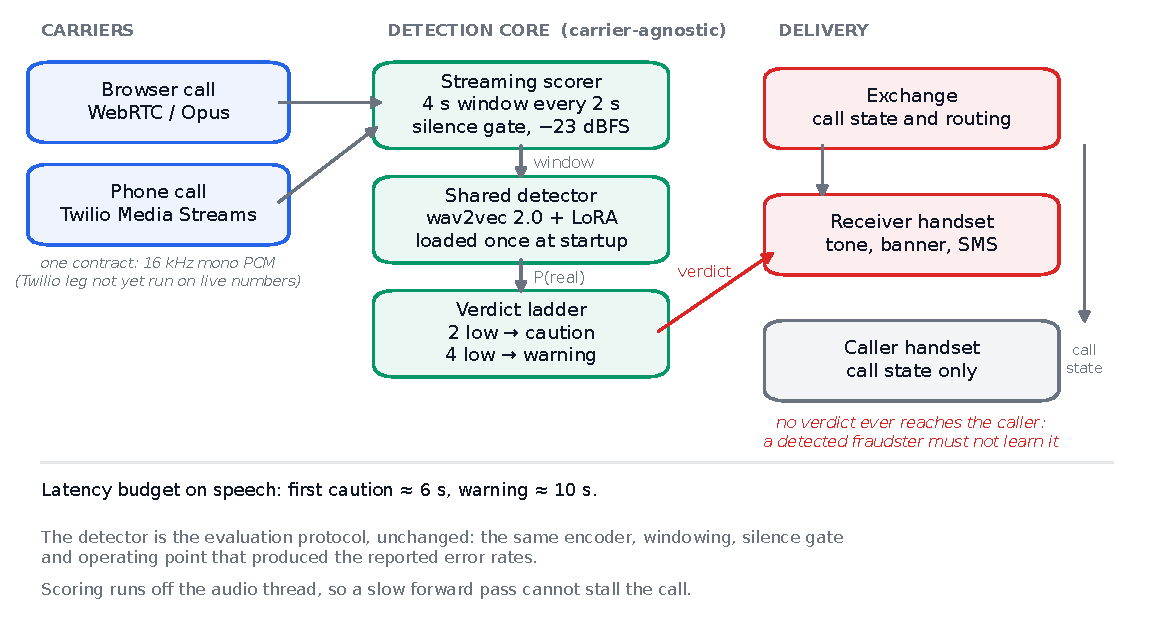
\includegraphics[width=\linewidth]{figures/system_architecture.pdf}
  \caption{The live-call detector. Two carriers, WebRTC and Twilio Media Streams,
  both resolve to the same 16\,kHz mono PCM contract, so the detection core is
  unaware of which one delivered the call. Verdicts travel only to the receiver's
  handset.}
  \label{fig:system}
\end{figure}

\subsubsection{Carriers}

Two carriers are implemented against one contract, a \texttt{PcmFrameSource} that
yields 16\,kHz mono float frames.

\emph{WebRTC} (\texttt{live\_call/webrtc\_harness/}) carries browser-to-browser
calls. The server is a participant in the call rather than a bystander: it accepts
an offer, subscribes to each peer's audio through a relay, and taps one copy for
detection while forwarding another to the other party. Audio tracks are keyed by
peer and dropped when that peer leaves; an earlier implementation accumulated every
past call's tracks in the room and eventually offered a new joiner more media lines
than its session description contained, which fails negotiation outright.

\emph{Twilio Media Streams} (\texttt{live\_call/media\_handler.py}) carries calls
from the public telephone network. Twilio opens a WebSocket and pushes base64
G.711 $\mu$-law at 8\,kHz; the handler decodes and resamples to the same contract.
Twilio's webhook requests are verified by HMAC signature; the media WebSocket itself is not
authenticated.

\subsubsection{Detection core}

One detector is shared by every call (\texttt{live\_call/detector.py}): the
checkpoint is loaded once at startup, not per call, because loading it inside the
first request added tens of seconds of silence to that call. Each call owns a
session (\texttt{live\_call/session.py}) that pulls frames, and the streaming scorer
(\texttt{src/inference/streaming.py}) applies the evaluation-time treatment: a
four-second window every two seconds, a $-50$\,dBFS silence gate so that pauses are
skipped rather than scored, and normalisation to $-23$\,dBFS.

Scoring happens on a worker thread. A slow forward pass must not stall the audio
path, because the carrier does not wait: frames arrive in real time whether or not
the previous window has finished.

\subsubsection{The escalation ladder}

A per-window score is too noisy to act on. The verdict engine
(\texttt{live\_call/verdict\_engine.py}) smooths the window scores (an exponential
moving average with weight 0.5) and requires agreement across consecutive smoothed
windows before it escalates:

\begin{itemize}
  \item \textbf{Listening} until two windows are scored.
  \item \textbf{Suspicious} after two consecutive windows below the threshold: an
    audible tone and a caution on the receiver's handset.
  \item \textbf{Likely cloned} after four: a spoken warning to the receiver's leg of
    the call and, on the telephone carrier, an SMS.
  \item Recovery after three consecutive windows at or above a bound halfway between
    the threshold and 1, so a single noisy stretch does not leave a call marked for its
    duration.
\end{itemize}

With a two-second hop this places the first caution near six seconds of speech and
the warning near ten. The asymmetry is deliberate: four windows to accuse, three to
forgive.

\subsubsection{Call state and routing}

The exchange (\texttt{live\_call/phone.py}) models a line as
\emph{idle}, \emph{ringing}, \emph{connected} or \emph{ended}, with the parties on
it. It holds no sockets and no audio, which makes the routing rule testable in
isolation: verdicts are addressed to the receiver's connection only, and the
caller's connection receives call state alone.

Two consequences of this design are worth recording because both were found by
running real calls rather than by reasoning about the code. First, monitoring starts
when the call is \emph{answered}, not when the caller's audio arrives; during
ringing the media path is still settling, and the resulting discontinuity scored as
two low windows and cautioned a genuine caller. Second, the receiver's audio path is
opened while the phone is ringing, so that the renegotiation it triggers completes
before anyone speaks.

\subsection{Interfaces}

A browser-based console presents both handsets, the signal path and the live
analysis on one screen; separate caller and receiver pages run the same code on two
devices. A dashboard exposes every scored window for inspection. The evaluation
endpoints (\texttt{/api/predict}, \texttt{/api/replay}) score a file through the
identical path, which is how the demonstration clips were verified; the operating point
was calibrated offline through the same scoring path (\texttt{src.inference.calibrate}).

\subsection{Verification}

The system is covered at three levels. Unit tests cover the exchange, the verdict
ladder, the windowing and the room bookkeeping. Integration tests drive the real
sockets. End-to-end tests place calls in a real browser against the loaded model and
assert the properties that matter: that a cloned caller raises the warning within
the budget, that a genuine caller raises nothing, that every two seconds of speech
produces a scored window, and that no verdict ever appears on the caller's side.

That last layer exists because the defects that mattered were all in the wiring
between components that each worked correctly alone. The most serious example: the
alert message carries its severity in one field and its delivery channel in another,
and the interface read the channel. Every unit test passed, the ladder escalated
correctly, the message was dispatched --- and no warning was ever displayed.

\subsection{What a caller meets}
\label{sec:system-calls}

Clip-level EER is not what a caller experiences. We replayed test clips through the live
scoring path (4\,s windows every 2\,s, smoothed, through the escalation ladder) and
stitched clips of one label into 60\,s calls. The final recipe's operating point was
chosen on the dev set by the rule used for the deployed model (the most sensitive setting
whose genuine 60\,s dev calls raise at most 5\% alerts of any level): a threshold of 0.687,
a caution after three fake-leaning windows and ``likely cloned'' after five; the same rule
reproduces the deployed model's published threshold exactly (Table~\ref{tab:calls}).

\begin{table}[t]
\centering
\caption{60\,s calls through the live path: share of genuine calls warned and of fake calls
caught, each meaning a caution or worse. Counts are small (6--41 calls per cell).}
\label{tab:calls}
\footnotesize
\setlength{\tabcolsep}{3pt}
\begin{tabular}{@{}lrrrr@{}}
\toprule
 & \multicolumn{2}{c}{Genuine warned} & \multicolumn{2}{c}{Fakes caught} \\
Test calls & Deployed & Final & Deployed & Final \\
\midrule
Evaluation pool (XTTS) & 0\% & 0\% & 100\% & 100\% \\
CM04 (Tortoise) & 0\% & 0\% & 33\% & 100\% \\
RVC test half & 0\% & 0\% & 100\% & 100\% \\
60 new speakers & 44\% & 0\% & 100\% & 100\% \\
IndicF5 & 0\% & 0\% & 67\% & 50\% \\
Chatterbox & 0\% & 0\% & 33\% & 17\% \\
HiACC, spontaneous & 100\% & 100\% & --- & --- \\
\bottomrule
\end{tabular}
% docs/results/live_final_recipe_v1.md
\end{table}

On read speech the final recipe is the better live model: it no longer warns genuine new
speakers (44\% of their calls to none) and it catches every Tortoise call (33\% to 100\%),
while catching fewer IndicF5 and Chatterbox calls. Spontaneous speech is worse at the call
level than per clip: one short clip replayed through the live ladder is rarely warned
(2.8\% final, 8.6\% deployed), but over
a minute its fake-leaning windows add up and every genuine spontaneous call is warned by
either model. Neither system should be put in front of spontaneous callers
before it has heard spontaneous genuine speech in training.

\subsection{Real phone calls}
\label{sec:real-calls}

Every result so far passes audio through a simulated line or a reference codec offline. As a
pilot on the real network, we made calls among ourselves, with written consent and our
faculty mentor's approval, over a commercial mobile network and recorded them on the receiving
handset, whose call recorder writes 8\,kHz mono AAC: 30 calls from three speakers. Twelve
calls are genuine and live, the speaker reading a prepared code-mixed script or talking freely;
six replay each speaker's own reading from a laptop loudspeaker into the calling phone; and
twelve replay clones of the same speakers saying the same scripts, made with XTTS-v2 (the seen
tool) and Chatterbox (an unseen one) from about 20\,s of reference speech. Genuine and cloned
replays share the loudspeaker path, so their comparison isolates the synthesis. Every replay
recording was matched back to the file played into it by the correlation of their
speech-activity tracks (0.54--0.95, against at most 0.40 for any other file), so no call
carries the wrong label. Each recording is scored offline through the live path at each
model's frozen operating point, as recorded and after a G.711 round trip (what the carrier
delivers); no threshold is chosen on these calls (\texttt{docs/real\_calls/PROTOCOL.md}).

\begin{table}[t]
\centering
\caption{Real mobile calls, scored as the carrier delivers them (G.711): number of calls warned
(caution or worse) and reaching ``likely cloned''. 30 calls from three speakers.}
\label{tab:realcalls}
\footnotesize
\setlength{\tabcolsep}{3pt}
\begin{tabular}{@{}lrrrr@{}}
\toprule
 & & Deployed & \multicolumn{2}{c}{Final recipe} \\
Calls & $n$ & likely cloned & warned & likely cloned \\
\midrule
Genuine, live & 12 & 8 & 3 & 1 \\
Genuine, replayed & 6 & 6 & 1 & 1 \\
XTTS-v2 clones, replayed & 6 & 6 & 5 & 5 \\
Chatterbox clones, replayed & 6 & 6 & 1 & 0 \\
\bottomrule
\end{tabular}
% docs/results/real_calls_v1.md
\end{table}

\textbf{The deployed model fails for two speakers of three.} It takes every replayed call,
genuine or cloned, to ``likely cloned'', and every live call of two speakers (mean window
scores 0.02--0.22 and below 0.001), but none of the third speaker's four live calls, which it
scores at 0.96--1.00 (Table~\ref{tab:realcalls}). Whether that speaker's voice or that speaker's
handset and network is the difference, three speakers cannot say. \textbf{The final recipe holds up on
the seen tool}: it warns three of twelve genuine live calls, one of them to ``likely cloned'',
all three the same speaker's calls; catches (takes to ``likely cloned'') five of six XTTS-v2
clone calls; and catches none of the six Chatterbox calls, of which it cautions one, matching
Chatterbox being the adapter's hardest unseen tool offline (Sec.~\ref{sec:res-chatterbox}).
Against the fair control, the genuine replays that share the clones' loudspeaker path, one of
six reaches ``likely cloned''; the window-level EER of the final recipe against them is 19.0\%
on XTTS-v2 and 50.0\% on Chatterbox. It is slower on real calls than offline for two speakers:
their three caught XTTS-v2 calls reach a caution 18--32\,s in and ``likely cloned'' 30--46\,s
in, where the five-window ladder could reach ``likely cloned'' after 12\,s; the third speaker's two are caught at
12 and 14\,s.

\textbf{The larger encoder does better on these calls.} SSL-AASIST fine-tuned on the
final-recipe data (Sec.~\ref{sec:res-finalssl}), at its own operating point chosen on the same
dev clips by the same rule (threshold 0.580, a caution after two fake-leaning windows and
``likely cloned'' after four), warns one of the twelve genuine live calls, a caution 48\,s in,
and takes none to ``likely cloned''. It takes all six XTTS-v2 calls to ``likely cloned'', four
of them 10--14\,s into the call, and of the Chatterbox calls it catches one and cautions two.
Against the genuine replays one of six reaches ``likely cloned'', as for the final recipe, and
its window-level EER against them is 4.4\% on XTTS-v2 and 36.6\% on Chatterbox. Its genuine
live calls show no early dip (mean 0.98 over the first 10\,s). Its shorter ladder makes it
faster and, by itself, more prone to false alarms, yet it warns fewer genuine calls. It is one
checkpoint, a retraining of seed 1234 kept for this test; GPU training does not repeat
exactly, and offline this one is the weakest of six trainings on Chatterbox (21.2\% against
8.2--18.3\%). On the held-out 60\,s calls that validate the operating points it warns no genuine
read-speech call and 11 of 41 genuine spontaneous calls (HiACC; one ``likely cloned''), where
the final recipe warns all 41; but trainings of this encoder differ on spontaneous speech
(Sec.~\ref{sec:res-finalssl}), so a second checkpoint must agree before it replaces the final
recipe.

\textbf{The final recipe's false alarms come early in a call.} Over the first 10\,s its mean
score on genuine live calls is 0.79, after 20\,s 0.98. Part of the cause is the first window,
which spans the quiet before the first word (median $-30$\,dBFS, against $-21$ to $-26$ for the
speech that follows): in eleven of the twelve calls it passes the $-50$\,dBFS gate, is normalised
and is scored as speech (mean 0.60), and the run of fake-leaning windows behind each warned genuine live call starts there.
Only part, though: replaying the calls with that window treated as silence, a diagnostic that
chooses nothing, clears two of the three warned genuine live calls over G.711, while as recorded
it clears one of four and cautions another; and one call over G.711 (two as recorded) still
reaches ``likely cloned'', its run including two speech windows 8--14\,s in.
A stricter speech gate at the start of a call would help but not suffice, and both it and the
operating point need real development calls, not these. The counts are small, and the intervals
say so: five of six clone calls caught is a 95\% Wilson interval of 44--97\%, none of six is
0--39\%, one of twelve genuine live calls ``likely cloned'' is 1.5--35\%.

\begin{figure}[t]
\centering
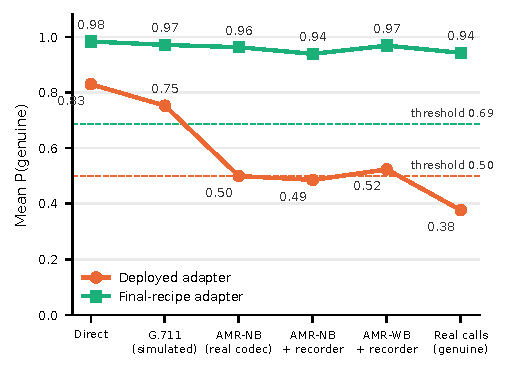
\includegraphics[width=\columnwidth]{figures/real_call_chain.pdf}
\caption{Mean P(genuine) of each speaker's direct recordings through the stages of a phone
call, and of the genuine live calls as the carrier delivers them. On average the deployed
adapter falls to its threshold at the mobile codec; the final recipe, trained through AMR-NB,
stays above its own. Dashed lines: each model's frozen live threshold.}
\label{fig:realchain}
\end{figure}

\textbf{The mobile codec is the largest single step in the deployed model's failure, for the
speakers it fails on.} We rebuilt the call chain on each speaker's direct recordings of the same
scripts, one stage at a time (Fig.~\ref{fig:realchain}). Averaged over the six readings, the
deployed model's mean P(genuine) falls from 0.83 on the direct recordings and 0.75 through the
simulated G.711 line to 0.50 through the reference AMR-NB codec, with the call recorder adding
little (0.49) and the 4G codec (AMR-WB) behaving alike (0.52). Per reading, two of the six cross
the threshold at AMR-NB (0.66 to 0.28 and 0.74 to 0.11), one stays above it (0.92 to 0.74),
one is below it before any codec (0.28), and the third speaker's two stay at 0.87--1.00 at
every stage, so the codec is the largest step for the speakers the model fails on, not a failure
of every voice. The final recipe stays at 0.82--1.00 through every stage for all six readings.
The real network costs the deployed model more still (0.38 on the genuine live calls, against
0.94 for the final recipe), but the direction is the one the offline AMR-NB results predicted
(Sec.~\ref{sec:res-new}). The final recipe changes two things at once, more voices and the real
codec, so these calls cannot separate them; offline, adding AMR-NB alone to the deployed
recipe's training recovers most of the codec loss (Sec.~\ref{sec:res-new}). The chain is
rebuilt by \texttt{src.inference.real\_call\_codecs}.

\subsection{Deployment status}

The WebRTC carrier is verified end to end against the deployed checkpoint. Each
demonstration clip was replayed through the live path and its behaviour recorded
rather than inferred from offline scores, because the two disagree: on a live call a
genuine caller can lose several consecutive windows that the same clip never loses
offline.

We tested the obvious explanation and it does not hold as far as we could test it.
An offline Opus~\cite{valin2012opus} round trip --- resample to 48\,kHz, encode and decode
with libsndfile's default encoder (not a browser's adaptive one), resample back --- and
rescoring through the identical streaming path leaves both genuine clips at zero windows
below the threshold, with a worst window of 0.984 against the 0.001 seen live. Both seen
attacks stay detected (the RVC clip loses 2 of 24 windows over G.711). An offline codec
round trip therefore does not reproduce the live degradation, and clone detection does
not depend on codec artefacts.\footnote{%
\texttt{docs/results/carrier\_effect\_v1.md}; reproduce with
\texttt{python -m src.inference.carrier\_sim}.}

The likeliest remaining causes are the real-time transport and the browser's own adaptive
encoder, which this test did not reproduce: jitter buffering, packet-loss concealment, or the bitrate adaptation a browser
applies while a connection is still settling. Concealment is the candidate we would
test first, because it synthesises audio to fill gaps, and a detector reporting that
machine-generated audio is not human would produce exactly this signature. That
remains untested. The call is negotiated at a high constant bitrate with
discontinuous transmission disabled, which is sensible for a demonstration, but the
dip survived that change and it should not be presented as the remedy.

The Twilio carrier is implemented and unit-tested but has not been verified on live
numbers, because the account's trial credit was exhausted. Real mobile calls have been
recorded on a handset and scored offline through the same path (Sec.~\ref{sec:real-calls}),
but the carrier itself, which would deliver those calls to the detector as they happen, is
the one leg not yet demonstrated end to end.
; label sec:system.
\section{System Design and Implementation}
\label{sec:system}

The evaluation protocol in Section~\ref{sec:method} scores four-second windows
of narrowband telephone audio. The deployed system is that protocol running on a
live call rather than on a manifest: the same encoder and the same four-second windows,
with an operating point calibrated on development calls through this path. The detector
itself does not change between the two, which is what lets a demonstration stand as
evidence rather than as illustration.

\subsection{Requirements}

Four requirements shaped the design, and each one rules out an otherwise obvious
implementation.

\textbf{The verdict must reach the callee and nobody else.} A system that tells the
caller they have been detected is a system that teaches attackers to evade it. This
is a routing requirement, and it is why call state is modelled explicitly rather
than broadcast to every participant of a session.

\textbf{The warning must arrive during the call.} A verdict delivered after the call
has ended protects nobody. This sets a latency budget rather than a throughput one:
the first credible warning must land within roughly ten seconds of speech.

\textbf{The audio the detector sees must be the audio it was trained on.} The
adapted model is trained on 8\,kHz G.711~\cite{itu1988g711} telephone audio, and its decision cue lives
in fine waveform structure (Section~\ref{sec:results}). Any resampling, codec or
level change between the carrier and the model is a domain shift.

\textbf{A single false alarm is more damaging than a missed clone.} The user is a
person receiving a call from someone they may know. The escalation ladder below is
built around that asymmetry.

\subsection{Architecture}

The system is a single Python service with three layers: carriers, which turn a call
into a stream of audio frames; a detection core, which is carrier-agnostic; and
delivery, which routes verdicts to the right participant.

\begin{figure}[t]
  \centering
  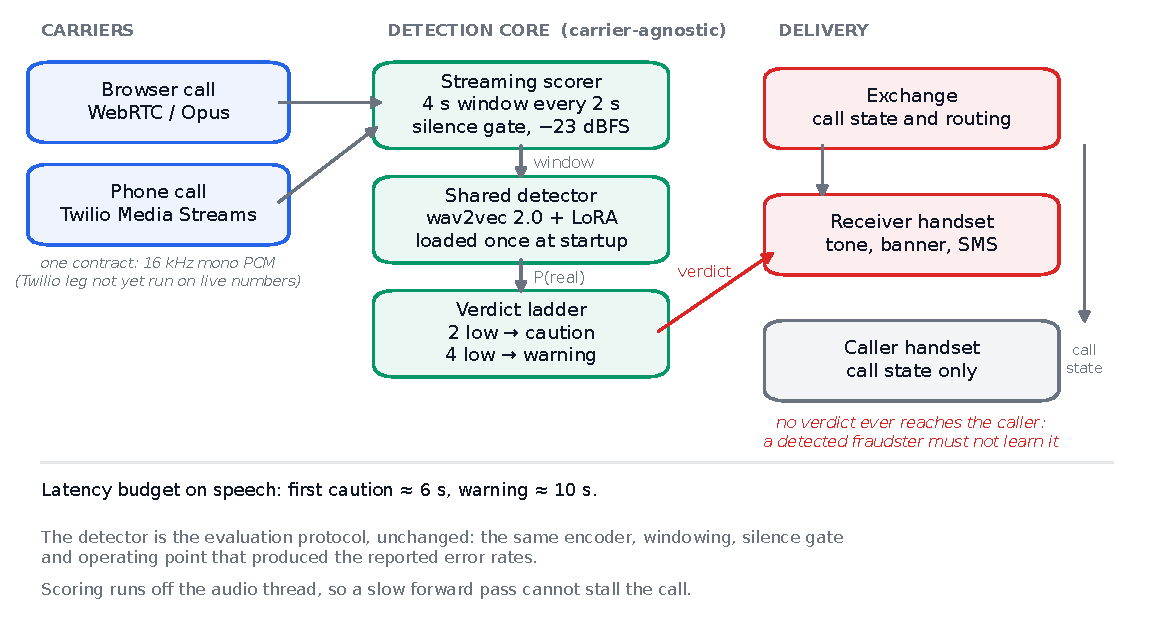
\includegraphics[width=\linewidth]{figures/system_architecture.pdf}
  \caption{The live-call detector. Two carriers, WebRTC and Twilio Media Streams,
  both resolve to the same 16\,kHz mono PCM contract, so the detection core is
  unaware of which one delivered the call. Verdicts travel only to the receiver's
  handset.}
  \label{fig:system}
\end{figure}

\subsubsection{Carriers}

Two carriers are implemented against one contract, a \texttt{PcmFrameSource} that
yields 16\,kHz mono float frames.

\emph{WebRTC} (\texttt{live\_call/webrtc\_harness/}) carries browser-to-browser
calls. The server is a participant in the call rather than a bystander: it accepts
an offer, subscribes to each peer's audio through a relay, and taps one copy for
detection while forwarding another to the other party. Audio tracks are keyed by
peer and dropped when that peer leaves; an earlier implementation accumulated every
past call's tracks in the room and eventually offered a new joiner more media lines
than its session description contained, which fails negotiation outright.

\emph{Twilio Media Streams} (\texttt{live\_call/media\_handler.py}) carries calls
from the public telephone network. Twilio opens a WebSocket and pushes base64
G.711 $\mu$-law at 8\,kHz; the handler decodes and resamples to the same contract.
Twilio's webhook requests are verified by HMAC signature; the media WebSocket itself is not
authenticated.

\subsubsection{Detection core}

One detector is shared by every call (\texttt{live\_call/detector.py}): the
checkpoint is loaded once at startup, not per call, because loading it inside the
first request added tens of seconds of silence to that call. Each call owns a
session (\texttt{live\_call/session.py}) that pulls frames, and the streaming scorer
(\texttt{src/inference/streaming.py}) applies the evaluation-time treatment: a
four-second window every two seconds, a $-50$\,dBFS silence gate so that pauses are
skipped rather than scored, and normalisation to $-23$\,dBFS.

Scoring happens on a worker thread. A slow forward pass must not stall the audio
path, because the carrier does not wait: frames arrive in real time whether or not
the previous window has finished.

\subsubsection{The escalation ladder}

A per-window score is too noisy to act on. The verdict engine
(\texttt{live\_call/verdict\_engine.py}) smooths the window scores (an exponential
moving average with weight 0.5) and requires agreement across consecutive smoothed
windows before it escalates:

\begin{itemize}
  \item \textbf{Listening} until two windows are scored.
  \item \textbf{Suspicious} after two consecutive windows below the threshold: an
    audible tone and a caution on the receiver's handset.
  \item \textbf{Likely cloned} after four: a spoken warning to the receiver's leg of
    the call and, on the telephone carrier, an SMS.
  \item Recovery after three consecutive windows at or above a bound halfway between
    the threshold and 1, so a single noisy stretch does not leave a call marked for its
    duration.
\end{itemize}

With a two-second hop this places the first caution near six seconds of speech and
the warning near ten. The asymmetry is deliberate: four windows to accuse, three to
forgive.

\subsubsection{Call state and routing}

The exchange (\texttt{live\_call/phone.py}) models a line as
\emph{idle}, \emph{ringing}, \emph{connected} or \emph{ended}, with the parties on
it. It holds no sockets and no audio, which makes the routing rule testable in
isolation: verdicts are addressed to the receiver's connection only, and the
caller's connection receives call state alone.

Two consequences of this design are worth recording because both were found by
running real calls rather than by reasoning about the code. First, monitoring starts
when the call is \emph{answered}, not when the caller's audio arrives; during
ringing the media path is still settling, and the resulting discontinuity scored as
two low windows and cautioned a genuine caller. Second, the receiver's audio path is
opened while the phone is ringing, so that the renegotiation it triggers completes
before anyone speaks.

\subsection{Interfaces}

A browser-based console presents both handsets, the signal path and the live
analysis on one screen; separate caller and receiver pages run the same code on two
devices. A dashboard exposes every scored window for inspection. The evaluation
endpoints (\texttt{/api/predict}, \texttt{/api/replay}) score a file through the
identical path, which is how the demonstration clips were verified; the operating point
was calibrated offline through the same scoring path (\texttt{src.inference.calibrate}).

\subsection{Verification}

The system is covered at three levels. Unit tests cover the exchange, the verdict
ladder, the windowing and the room bookkeeping. Integration tests drive the real
sockets. End-to-end tests place calls in a real browser against the loaded model and
assert the properties that matter: that a cloned caller raises the warning within
the budget, that a genuine caller raises nothing, that every two seconds of speech
produces a scored window, and that no verdict ever appears on the caller's side.

That last layer exists because the defects that mattered were all in the wiring
between components that each worked correctly alone. The most serious example: the
alert message carries its severity in one field and its delivery channel in another,
and the interface read the channel. Every unit test passed, the ladder escalated
correctly, the message was dispatched --- and no warning was ever displayed.

\subsection{What a caller meets}
\label{sec:system-calls}

Clip-level EER is not what a caller experiences. We replayed test clips through the live
scoring path (4\,s windows every 2\,s, smoothed, through the escalation ladder) and
stitched clips of one label into 60\,s calls. The final recipe's operating point was
chosen on the dev set by the rule used for the deployed model (the most sensitive setting
whose genuine 60\,s dev calls raise at most 5\% alerts of any level): a threshold of 0.687,
a caution after three fake-leaning windows and ``likely cloned'' after five; the same rule
reproduces the deployed model's published threshold exactly (Table~\ref{tab:calls}).

\begin{table}[t]
\centering
\caption{60\,s calls through the live path: share of genuine calls warned and of fake calls
caught, each meaning a caution or worse. Counts are small (6--41 calls per cell).}
\label{tab:calls}
\footnotesize
\setlength{\tabcolsep}{3pt}
\begin{tabular}{@{}lrrrr@{}}
\toprule
 & \multicolumn{2}{c}{Genuine warned} & \multicolumn{2}{c}{Fakes caught} \\
Test calls & Deployed & Final & Deployed & Final \\
\midrule
Evaluation pool (XTTS) & 0\% & 0\% & 100\% & 100\% \\
CM04 (Tortoise) & 0\% & 0\% & 33\% & 100\% \\
RVC test half & 0\% & 0\% & 100\% & 100\% \\
60 new speakers & 44\% & 0\% & 100\% & 100\% \\
IndicF5 & 0\% & 0\% & 67\% & 50\% \\
Chatterbox & 0\% & 0\% & 33\% & 17\% \\
HiACC, spontaneous & 100\% & 100\% & --- & --- \\
\bottomrule
\end{tabular}
% docs/results/live_final_recipe_v1.md
\end{table}

On read speech the final recipe is the better live model: it no longer warns genuine new
speakers (44\% of their calls to none) and it catches every Tortoise call (33\% to 100\%),
while catching fewer IndicF5 and Chatterbox calls. Spontaneous speech is worse at the call
level than per clip: one short clip replayed through the live ladder is rarely warned
(2.8\% final, 8.6\% deployed), but over
a minute its fake-leaning windows add up and every genuine spontaneous call is warned by
either model. Neither system should be put in front of spontaneous callers
before it has heard spontaneous genuine speech in training.

\subsection{Real phone calls}
\label{sec:real-calls}

Every result so far passes audio through a simulated line or a reference codec offline. As a
pilot on the real network, we made calls among ourselves, with written consent and our
faculty mentor's approval, over a commercial mobile network and recorded them on the receiving
handset, whose call recorder writes 8\,kHz mono AAC: 30 calls from three speakers. Twelve
calls are genuine and live, the speaker reading a prepared code-mixed script or talking freely;
six replay each speaker's own reading from a laptop loudspeaker into the calling phone; and
twelve replay clones of the same speakers saying the same scripts, made with XTTS-v2 (the seen
tool) and Chatterbox (an unseen one) from about 20\,s of reference speech. Genuine and cloned
replays share the loudspeaker path, so their comparison isolates the synthesis. Every replay
recording was matched back to the file played into it by the correlation of their
speech-activity tracks (0.54--0.95, against at most 0.40 for any other file), so no call
carries the wrong label. Each recording is scored offline through the live path at each
model's frozen operating point, as recorded and after a G.711 round trip (what the carrier
delivers); no threshold is chosen on these calls (\texttt{docs/real\_calls/PROTOCOL.md}).

\begin{table}[t]
\centering
\caption{Real mobile calls, scored as the carrier delivers them (G.711): number of calls warned
(caution or worse) and reaching ``likely cloned''. 30 calls from three speakers.}
\label{tab:realcalls}
\footnotesize
\setlength{\tabcolsep}{3pt}
\begin{tabular}{@{}lrrrr@{}}
\toprule
 & & Deployed & \multicolumn{2}{c}{Final recipe} \\
Calls & $n$ & likely cloned & warned & likely cloned \\
\midrule
Genuine, live & 12 & 8 & 3 & 1 \\
Genuine, replayed & 6 & 6 & 1 & 1 \\
XTTS-v2 clones, replayed & 6 & 6 & 5 & 5 \\
Chatterbox clones, replayed & 6 & 6 & 1 & 0 \\
\bottomrule
\end{tabular}
% docs/results/real_calls_v1.md
\end{table}

\textbf{The deployed model fails for two speakers of three.} It takes every replayed call,
genuine or cloned, to ``likely cloned'', and every live call of two speakers (mean window
scores 0.02--0.22 and below 0.001), but none of the third speaker's four live calls, which it
scores at 0.96--1.00 (Table~\ref{tab:realcalls}). Whether that speaker's voice or that speaker's
handset and network is the difference, three speakers cannot say. \textbf{The final recipe holds up on
the seen tool}: it warns three of twelve genuine live calls, one of them to ``likely cloned'',
all three the same speaker's calls; catches (takes to ``likely cloned'') five of six XTTS-v2
clone calls; and catches none of the six Chatterbox calls, of which it cautions one, matching
Chatterbox being the adapter's hardest unseen tool offline (Sec.~\ref{sec:res-chatterbox}).
Against the fair control, the genuine replays that share the clones' loudspeaker path, one of
six reaches ``likely cloned''; the window-level EER of the final recipe against them is 19.0\%
on XTTS-v2 and 50.0\% on Chatterbox. It is slower on real calls than offline for two speakers:
their three caught XTTS-v2 calls reach a caution 18--32\,s in and ``likely cloned'' 30--46\,s
in, where the five-window ladder could reach ``likely cloned'' after 12\,s; the third speaker's two are caught at
12 and 14\,s.

\textbf{The larger encoder does better on these calls.} SSL-AASIST fine-tuned on the
final-recipe data (Sec.~\ref{sec:res-finalssl}), at its own operating point chosen on the same
dev clips by the same rule (threshold 0.580, a caution after two fake-leaning windows and
``likely cloned'' after four), warns one of the twelve genuine live calls, a caution 48\,s in,
and takes none to ``likely cloned''. It takes all six XTTS-v2 calls to ``likely cloned'', four
of them 10--14\,s into the call, and of the Chatterbox calls it catches one and cautions two.
Against the genuine replays one of six reaches ``likely cloned'', as for the final recipe, and
its window-level EER against them is 4.4\% on XTTS-v2 and 36.6\% on Chatterbox. Its genuine
live calls show no early dip (mean 0.98 over the first 10\,s). Its shorter ladder makes it
faster and, by itself, more prone to false alarms, yet it warns fewer genuine calls. It is one
checkpoint, a retraining of seed 1234 kept for this test; GPU training does not repeat
exactly, and offline this one is the weakest of six trainings on Chatterbox (21.2\% against
8.2--18.3\%). On the held-out 60\,s calls that validate the operating points it warns no genuine
read-speech call and 11 of 41 genuine spontaneous calls (HiACC; one ``likely cloned''), where
the final recipe warns all 41; but trainings of this encoder differ on spontaneous speech
(Sec.~\ref{sec:res-finalssl}), so a second checkpoint must agree before it replaces the final
recipe.

\textbf{The final recipe's false alarms come early in a call.} Over the first 10\,s its mean
score on genuine live calls is 0.79, after 20\,s 0.98. Part of the cause is the first window,
which spans the quiet before the first word (median $-30$\,dBFS, against $-21$ to $-26$ for the
speech that follows): in eleven of the twelve calls it passes the $-50$\,dBFS gate, is normalised
and is scored as speech (mean 0.60), and the run of fake-leaning windows behind each warned genuine live call starts there.
Only part, though: replaying the calls with that window treated as silence, a diagnostic that
chooses nothing, clears two of the three warned genuine live calls over G.711, while as recorded
it clears one of four and cautions another; and one call over G.711 (two as recorded) still
reaches ``likely cloned'', its run including two speech windows 8--14\,s in.
A stricter speech gate at the start of a call would help but not suffice, and both it and the
operating point need real development calls, not these. The counts are small, and the intervals
say so: five of six clone calls caught is a 95\% Wilson interval of 44--97\%, none of six is
0--39\%, one of twelve genuine live calls ``likely cloned'' is 1.5--35\%.

\begin{figure}[t]
\centering
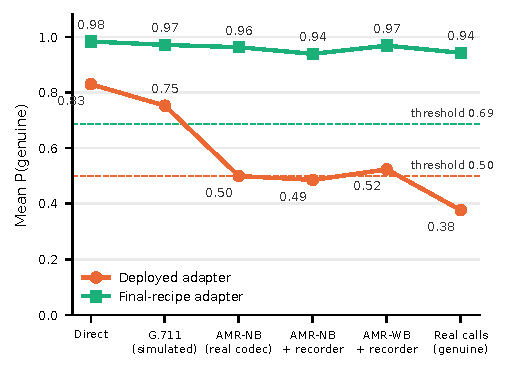
\includegraphics[width=\columnwidth]{figures/real_call_chain.pdf}
\caption{Mean P(genuine) of each speaker's direct recordings through the stages of a phone
call, and of the genuine live calls as the carrier delivers them. On average the deployed
adapter falls to its threshold at the mobile codec; the final recipe, trained through AMR-NB,
stays above its own. Dashed lines: each model's frozen live threshold.}
\label{fig:realchain}
\end{figure}

\textbf{The mobile codec is the largest single step in the deployed model's failure, for the
speakers it fails on.} We rebuilt the call chain on each speaker's direct recordings of the same
scripts, one stage at a time (Fig.~\ref{fig:realchain}). Averaged over the six readings, the
deployed model's mean P(genuine) falls from 0.83 on the direct recordings and 0.75 through the
simulated G.711 line to 0.50 through the reference AMR-NB codec, with the call recorder adding
little (0.49) and the 4G codec (AMR-WB) behaving alike (0.52). Per reading, two of the six cross
the threshold at AMR-NB (0.66 to 0.28 and 0.74 to 0.11), one stays above it (0.92 to 0.74),
one is below it before any codec (0.28), and the third speaker's two stay at 0.87--1.00 at
every stage, so the codec is the largest step for the speakers the model fails on, not a failure
of every voice. The final recipe stays at 0.82--1.00 through every stage for all six readings.
The real network costs the deployed model more still (0.38 on the genuine live calls, against
0.94 for the final recipe), but the direction is the one the offline AMR-NB results predicted
(Sec.~\ref{sec:res-new}). The final recipe changes two things at once, more voices and the real
codec, so these calls cannot separate them; offline, adding AMR-NB alone to the deployed
recipe's training recovers most of the codec loss (Sec.~\ref{sec:res-new}). The chain is
rebuilt by \texttt{src.inference.real\_call\_codecs}.

\subsection{Deployment status}

The WebRTC carrier is verified end to end against the deployed checkpoint. Each
demonstration clip was replayed through the live path and its behaviour recorded
rather than inferred from offline scores, because the two disagree: on a live call a
genuine caller can lose several consecutive windows that the same clip never loses
offline.

We tested the obvious explanation and it does not hold as far as we could test it.
An offline Opus~\cite{valin2012opus} round trip --- resample to 48\,kHz, encode and decode
with libsndfile's default encoder (not a browser's adaptive one), resample back --- and
rescoring through the identical streaming path leaves both genuine clips at zero windows
below the threshold, with a worst window of 0.984 against the 0.001 seen live. Both seen
attacks stay detected (the RVC clip loses 2 of 24 windows over G.711). An offline codec
round trip therefore does not reproduce the live degradation, and clone detection does
not depend on codec artefacts.\footnote{%
\texttt{docs/results/carrier\_effect\_v1.md}; reproduce with
\texttt{python -m src.inference.carrier\_sim}.}

The likeliest remaining causes are the real-time transport and the browser's own adaptive
encoder, which this test did not reproduce: jitter buffering, packet-loss concealment, or the bitrate adaptation a browser
applies while a connection is still settling. Concealment is the candidate we would
test first, because it synthesises audio to fill gaps, and a detector reporting that
machine-generated audio is not human would produce exactly this signature. That
remains untested. The call is negotiated at a high constant bitrate with
discontinuous transmission disabled, which is sensible for a demonstration, but the
dip survived that change and it should not be presented as the remedy.

The Twilio carrier is implemented and unit-tested but has not been verified on live
numbers, because the account's trial credit was exhausted. Real mobile calls have been
recorded on a handset and scored offline through the same path (Sec.~\ref{sec:real-calls}),
but the carrier itself, which would deliver those calls to the detector as they happen, is
the one leg not yet demonstrated end to end.
; label sec:system.
\section{System Design and Implementation}
\label{sec:system}

The evaluation protocol in Section~\ref{sec:method} scores four-second windows
of narrowband telephone audio. The deployed system is that protocol running on a
live call rather than on a manifest: the same encoder and the same four-second windows,
with an operating point calibrated on development calls through this path. The detector
itself does not change between the two, which is what lets a demonstration stand as
evidence rather than as illustration.

\subsection{Requirements}

Four requirements shaped the design, and each one rules out an otherwise obvious
implementation.

\textbf{The verdict must reach the callee and nobody else.} A system that tells the
caller they have been detected is a system that teaches attackers to evade it. This
is a routing requirement, and it is why call state is modelled explicitly rather
than broadcast to every participant of a session.

\textbf{The warning must arrive during the call.} A verdict delivered after the call
has ended protects nobody. This sets a latency budget rather than a throughput one:
the first credible warning must land within roughly ten seconds of speech.

\textbf{The audio the detector sees must be the audio it was trained on.} The
adapted model is trained on 8\,kHz G.711~\cite{itu1988g711} telephone audio, and its decision cue lives
in fine waveform structure (Section~\ref{sec:results}). Any resampling, codec or
level change between the carrier and the model is a domain shift.

\textbf{A single false alarm is more damaging than a missed clone.} The user is a
person receiving a call from someone they may know. The escalation ladder below is
built around that asymmetry.

\subsection{Architecture}

The system is a single Python service with three layers: carriers, which turn a call
into a stream of audio frames; a detection core, which is carrier-agnostic; and
delivery, which routes verdicts to the right participant.

\begin{figure}[t]
  \centering
  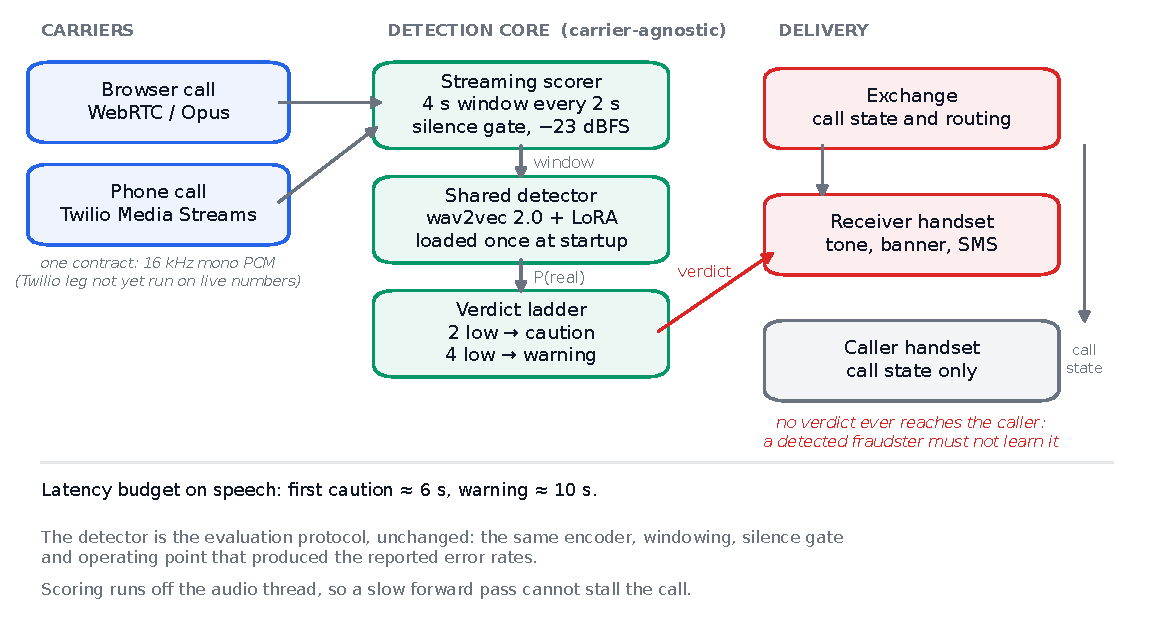
\includegraphics[width=\linewidth]{figures/system_architecture.pdf}
  \caption{The live-call detector. Two carriers, WebRTC and Twilio Media Streams,
  both resolve to the same 16\,kHz mono PCM contract, so the detection core is
  unaware of which one delivered the call. Verdicts travel only to the receiver's
  handset.}
  \label{fig:system}
\end{figure}

\subsubsection{Carriers}

Two carriers are implemented against one contract, a \texttt{PcmFrameSource} that
yields 16\,kHz mono float frames.

\emph{WebRTC} (\texttt{live\_call/webrtc\_harness/}) carries browser-to-browser
calls. The server is a participant in the call rather than a bystander: it accepts
an offer, subscribes to each peer's audio through a relay, and taps one copy for
detection while forwarding another to the other party. Audio tracks are keyed by
peer and dropped when that peer leaves; an earlier implementation accumulated every
past call's tracks in the room and eventually offered a new joiner more media lines
than its session description contained, which fails negotiation outright.

\emph{Twilio Media Streams} (\texttt{live\_call/media\_handler.py}) carries calls
from the public telephone network. Twilio opens a WebSocket and pushes base64
G.711 $\mu$-law at 8\,kHz; the handler decodes and resamples to the same contract.
Twilio's webhook requests are verified by HMAC signature; the media WebSocket itself is not
authenticated.

\subsubsection{Detection core}

One detector is shared by every call (\texttt{live\_call/detector.py}): the
checkpoint is loaded once at startup, not per call, because loading it inside the
first request added tens of seconds of silence to that call. Each call owns a
session (\texttt{live\_call/session.py}) that pulls frames, and the streaming scorer
(\texttt{src/inference/streaming.py}) applies the evaluation-time treatment: a
four-second window every two seconds, a $-50$\,dBFS silence gate so that pauses are
skipped rather than scored, and normalisation to $-23$\,dBFS.

Scoring happens on a worker thread. A slow forward pass must not stall the audio
path, because the carrier does not wait: frames arrive in real time whether or not
the previous window has finished.

\subsubsection{The escalation ladder}

A per-window score is too noisy to act on. The verdict engine
(\texttt{live\_call/verdict\_engine.py}) smooths the window scores (an exponential
moving average with weight 0.5) and requires agreement across consecutive smoothed
windows before it escalates:

\begin{itemize}
  \item \textbf{Listening} until two windows are scored.
  \item \textbf{Suspicious} after two consecutive windows below the threshold: an
    audible tone and a caution on the receiver's handset.
  \item \textbf{Likely cloned} after four: a spoken warning to the receiver's leg of
    the call and, on the telephone carrier, an SMS.
  \item Recovery after three consecutive windows at or above a bound halfway between
    the threshold and 1, so a single noisy stretch does not leave a call marked for its
    duration.
\end{itemize}

With a two-second hop this places the first caution near six seconds of speech and
the warning near ten. The asymmetry is deliberate: four windows to accuse, three to
forgive.

\subsubsection{Call state and routing}

The exchange (\texttt{live\_call/phone.py}) models a line as
\emph{idle}, \emph{ringing}, \emph{connected} or \emph{ended}, with the parties on
it. It holds no sockets and no audio, which makes the routing rule testable in
isolation: verdicts are addressed to the receiver's connection only, and the
caller's connection receives call state alone.

Two consequences of this design are worth recording because both were found by
running real calls rather than by reasoning about the code. First, monitoring starts
when the call is \emph{answered}, not when the caller's audio arrives; during
ringing the media path is still settling, and the resulting discontinuity scored as
two low windows and cautioned a genuine caller. Second, the receiver's audio path is
opened while the phone is ringing, so that the renegotiation it triggers completes
before anyone speaks.

\subsection{Interfaces}

A browser-based console presents both handsets, the signal path and the live
analysis on one screen; separate caller and receiver pages run the same code on two
devices. A dashboard exposes every scored window for inspection. The evaluation
endpoints (\texttt{/api/predict}, \texttt{/api/replay}) score a file through the
identical path, which is how the demonstration clips were verified; the operating point
was calibrated offline through the same scoring path (\texttt{src.inference.calibrate}).

\subsection{Verification}

The system is covered at three levels. Unit tests cover the exchange, the verdict
ladder, the windowing and the room bookkeeping. Integration tests drive the real
sockets. End-to-end tests place calls in a real browser against the loaded model and
assert the properties that matter: that a cloned caller raises the warning within
the budget, that a genuine caller raises nothing, that every two seconds of speech
produces a scored window, and that no verdict ever appears on the caller's side.

That last layer exists because the defects that mattered were all in the wiring
between components that each worked correctly alone. The most serious example: the
alert message carries its severity in one field and its delivery channel in another,
and the interface read the channel. Every unit test passed, the ladder escalated
correctly, the message was dispatched --- and no warning was ever displayed.

\subsection{What a caller meets}
\label{sec:system-calls}

Clip-level EER is not what a caller experiences. We replayed test clips through the live
scoring path (4\,s windows every 2\,s, smoothed, through the escalation ladder) and
stitched clips of one label into 60\,s calls. The final recipe's operating point was
chosen on the dev set by the rule used for the deployed model (the most sensitive setting
whose genuine 60\,s dev calls raise at most 5\% alerts of any level): a threshold of 0.687,
a caution after three fake-leaning windows and ``likely cloned'' after five; the same rule
reproduces the deployed model's published threshold exactly (Table~\ref{tab:calls}).

\begin{table}[t]
\centering
\caption{60\,s calls through the live path: share of genuine calls warned and of fake calls
caught, each meaning a caution or worse. Counts are small (6--41 calls per cell).}
\label{tab:calls}
\footnotesize
\setlength{\tabcolsep}{3pt}
\begin{tabular}{@{}lrrrr@{}}
\toprule
 & \multicolumn{2}{c}{Genuine warned} & \multicolumn{2}{c}{Fakes caught} \\
Test calls & Deployed & Final & Deployed & Final \\
\midrule
Evaluation pool (XTTS) & 0\% & 0\% & 100\% & 100\% \\
CM04 (Tortoise) & 0\% & 0\% & 33\% & 100\% \\
RVC test half & 0\% & 0\% & 100\% & 100\% \\
60 new speakers & 44\% & 0\% & 100\% & 100\% \\
IndicF5 & 0\% & 0\% & 67\% & 50\% \\
Chatterbox & 0\% & 0\% & 33\% & 17\% \\
HiACC, spontaneous & 100\% & 100\% & --- & --- \\
\bottomrule
\end{tabular}
% docs/results/live_final_recipe_v1.md
\end{table}

On read speech the final recipe is the better live model: it no longer warns genuine new
speakers (44\% of their calls to none) and it catches every Tortoise call (33\% to 100\%),
while catching fewer IndicF5 and Chatterbox calls. Spontaneous speech is worse at the call
level than per clip: one short clip replayed through the live ladder is rarely warned
(2.8\% final, 8.6\% deployed), but over
a minute its fake-leaning windows add up and every genuine spontaneous call is warned by
either model. Neither system should be put in front of spontaneous callers
before it has heard spontaneous genuine speech in training.

\subsection{Real phone calls}
\label{sec:real-calls}

Every result so far passes audio through a simulated line or a reference codec offline. As a
pilot on the real network, we made calls among ourselves, with written consent and our
faculty mentor's approval, over a commercial mobile network and recorded them on the receiving
handset, whose call recorder writes 8\,kHz mono AAC: 30 calls from three speakers. Twelve
calls are genuine and live, the speaker reading a prepared code-mixed script or talking freely;
six replay each speaker's own reading from a laptop loudspeaker into the calling phone; and
twelve replay clones of the same speakers saying the same scripts, made with XTTS-v2 (the seen
tool) and Chatterbox (an unseen one) from about 20\,s of reference speech. Genuine and cloned
replays share the loudspeaker path, so their comparison isolates the synthesis. Every replay
recording was matched back to the file played into it by the correlation of their
speech-activity tracks (0.54--0.95, against at most 0.40 for any other file), so no call
carries the wrong label. Each recording is scored offline through the live path at each
model's frozen operating point, as recorded and after a G.711 round trip (what the carrier
delivers); no threshold is chosen on these calls (\texttt{docs/real\_calls/PROTOCOL.md}).

\begin{table}[t]
\centering
\caption{Real mobile calls, scored as the carrier delivers them (G.711): number of calls warned
(caution or worse) and reaching ``likely cloned''. 30 calls from three speakers.}
\label{tab:realcalls}
\footnotesize
\setlength{\tabcolsep}{3pt}
\begin{tabular}{@{}lrrrr@{}}
\toprule
 & & Deployed & \multicolumn{2}{c}{Final recipe} \\
Calls & $n$ & likely cloned & warned & likely cloned \\
\midrule
Genuine, live & 12 & 8 & 3 & 1 \\
Genuine, replayed & 6 & 6 & 1 & 1 \\
XTTS-v2 clones, replayed & 6 & 6 & 5 & 5 \\
Chatterbox clones, replayed & 6 & 6 & 1 & 0 \\
\bottomrule
\end{tabular}
% docs/results/real_calls_v1.md
\end{table}

\textbf{The deployed model fails for two speakers of three.} It takes every replayed call,
genuine or cloned, to ``likely cloned'', and every live call of two speakers (mean window
scores 0.02--0.22 and below 0.001), but none of the third speaker's four live calls, which it
scores at 0.96--1.00 (Table~\ref{tab:realcalls}). Whether that speaker's voice or that speaker's
handset and network is the difference, three speakers cannot say. \textbf{The final recipe holds up on
the seen tool}: it warns three of twelve genuine live calls, one of them to ``likely cloned'',
all three the same speaker's calls; catches (takes to ``likely cloned'') five of six XTTS-v2
clone calls; and catches none of the six Chatterbox calls, of which it cautions one, matching
Chatterbox being the adapter's hardest unseen tool offline (Sec.~\ref{sec:res-chatterbox}).
Against the fair control, the genuine replays that share the clones' loudspeaker path, one of
six reaches ``likely cloned''; the window-level EER of the final recipe against them is 19.0\%
on XTTS-v2 and 50.0\% on Chatterbox. It is slower on real calls than offline for two speakers:
their three caught XTTS-v2 calls reach a caution 18--32\,s in and ``likely cloned'' 30--46\,s
in, where the five-window ladder could reach ``likely cloned'' after 12\,s; the third speaker's two are caught at
12 and 14\,s.

\textbf{The larger encoder does better on these calls.} SSL-AASIST fine-tuned on the
final-recipe data (Sec.~\ref{sec:res-finalssl}), at its own operating point chosen on the same
dev clips by the same rule (threshold 0.580, a caution after two fake-leaning windows and
``likely cloned'' after four), warns one of the twelve genuine live calls, a caution 48\,s in,
and takes none to ``likely cloned''. It takes all six XTTS-v2 calls to ``likely cloned'', four
of them 10--14\,s into the call, and of the Chatterbox calls it catches one and cautions two.
Against the genuine replays one of six reaches ``likely cloned'', as for the final recipe, and
its window-level EER against them is 4.4\% on XTTS-v2 and 36.6\% on Chatterbox. Its genuine
live calls show no early dip (mean 0.98 over the first 10\,s). Its shorter ladder makes it
faster and, by itself, more prone to false alarms, yet it warns fewer genuine calls. It is one
checkpoint, a retraining of seed 1234 kept for this test; GPU training does not repeat
exactly, and offline this one is the weakest of six trainings on Chatterbox (21.2\% against
8.2--18.3\%). On the held-out 60\,s calls that validate the operating points it warns no genuine
read-speech call and 11 of 41 genuine spontaneous calls (HiACC; one ``likely cloned''), where
the final recipe warns all 41; but trainings of this encoder differ on spontaneous speech
(Sec.~\ref{sec:res-finalssl}), so a second checkpoint must agree before it replaces the final
recipe.

\textbf{The final recipe's false alarms come early in a call.} Over the first 10\,s its mean
score on genuine live calls is 0.79, after 20\,s 0.98. Part of the cause is the first window,
which spans the quiet before the first word (median $-30$\,dBFS, against $-21$ to $-26$ for the
speech that follows): in eleven of the twelve calls it passes the $-50$\,dBFS gate, is normalised
and is scored as speech (mean 0.60), and the run of fake-leaning windows behind each warned genuine live call starts there.
Only part, though: replaying the calls with that window treated as silence, a diagnostic that
chooses nothing, clears two of the three warned genuine live calls over G.711, while as recorded
it clears one of four and cautions another; and one call over G.711 (two as recorded) still
reaches ``likely cloned'', its run including two speech windows 8--14\,s in.
A stricter speech gate at the start of a call would help but not suffice, and both it and the
operating point need real development calls, not these. The counts are small, and the intervals
say so: five of six clone calls caught is a 95\% Wilson interval of 44--97\%, none of six is
0--39\%, one of twelve genuine live calls ``likely cloned'' is 1.5--35\%.

\begin{figure}[t]
\centering
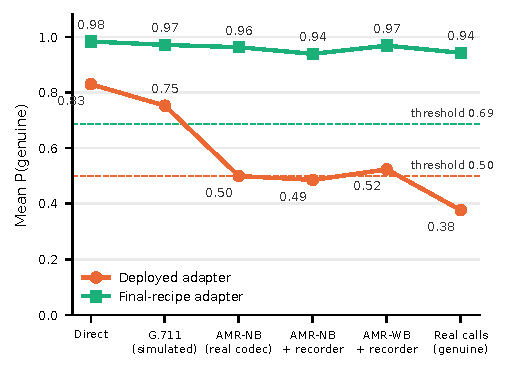
\includegraphics[width=\columnwidth]{figures/real_call_chain.pdf}
\caption{Mean P(genuine) of each speaker's direct recordings through the stages of a phone
call, and of the genuine live calls as the carrier delivers them. On average the deployed
adapter falls to its threshold at the mobile codec; the final recipe, trained through AMR-NB,
stays above its own. Dashed lines: each model's frozen live threshold.}
\label{fig:realchain}
\end{figure}

\textbf{The mobile codec is the largest single step in the deployed model's failure, for the
speakers it fails on.} We rebuilt the call chain on each speaker's direct recordings of the same
scripts, one stage at a time (Fig.~\ref{fig:realchain}). Averaged over the six readings, the
deployed model's mean P(genuine) falls from 0.83 on the direct recordings and 0.75 through the
simulated G.711 line to 0.50 through the reference AMR-NB codec, with the call recorder adding
little (0.49) and the 4G codec (AMR-WB) behaving alike (0.52). Per reading, two of the six cross
the threshold at AMR-NB (0.66 to 0.28 and 0.74 to 0.11), one stays above it (0.92 to 0.74),
one is below it before any codec (0.28), and the third speaker's two stay at 0.87--1.00 at
every stage, so the codec is the largest step for the speakers the model fails on, not a failure
of every voice. The final recipe stays at 0.82--1.00 through every stage for all six readings.
The real network costs the deployed model more still (0.38 on the genuine live calls, against
0.94 for the final recipe), but the direction is the one the offline AMR-NB results predicted
(Sec.~\ref{sec:res-new}). The final recipe changes two things at once, more voices and the real
codec, so these calls cannot separate them; offline, adding AMR-NB alone to the deployed
recipe's training recovers most of the codec loss (Sec.~\ref{sec:res-new}). The chain is
rebuilt by \texttt{src.inference.real\_call\_codecs}.

\subsection{Deployment status}

The WebRTC carrier is verified end to end against the deployed checkpoint. Each
demonstration clip was replayed through the live path and its behaviour recorded
rather than inferred from offline scores, because the two disagree: on a live call a
genuine caller can lose several consecutive windows that the same clip never loses
offline.

We tested the obvious explanation and it does not hold as far as we could test it.
An offline Opus~\cite{valin2012opus} round trip --- resample to 48\,kHz, encode and decode
with libsndfile's default encoder (not a browser's adaptive one), resample back --- and
rescoring through the identical streaming path leaves both genuine clips at zero windows
below the threshold, with a worst window of 0.984 against the 0.001 seen live. Both seen
attacks stay detected (the RVC clip loses 2 of 24 windows over G.711). An offline codec
round trip therefore does not reproduce the live degradation, and clone detection does
not depend on codec artefacts.\footnote{%
\texttt{docs/results/carrier\_effect\_v1.md}; reproduce with
\texttt{python -m src.inference.carrier\_sim}.}

The likeliest remaining causes are the real-time transport and the browser's own adaptive
encoder, which this test did not reproduce: jitter buffering, packet-loss concealment, or the bitrate adaptation a browser
applies while a connection is still settling. Concealment is the candidate we would
test first, because it synthesises audio to fill gaps, and a detector reporting that
machine-generated audio is not human would produce exactly this signature. That
remains untested. The call is negotiated at a high constant bitrate with
discontinuous transmission disabled, which is sensible for a demonstration, but the
dip survived that change and it should not be presented as the remedy.

The Twilio carrier is implemented and unit-tested but has not been verified on live
numbers, because the account's trial credit was exhausted. Real mobile calls have been
recorded on a handset and scored offline through the same path (Sec.~\ref{sec:real-calls}),
but the carrier itself, which would deliver those calls to the detector as they happen, is
the one leg not yet demonstrated end to end.
           % SK: live call system, label sec:system
% Conclusion and future work (owner SK). The limitations section is deliberately
% longer than the contributions section; every item in it is measured, not feared.
\section{Conclusion and Future Work}
\label{sec:conclusion}

An English-trained deepfake detector that reaches 0.85\% EER on ASVspoof does not
work on Hindi--English telephone speech. It reaches 48.21\% EER on clean code-mixed
audio and 58.42\% over the channel, with AUC below chance in the channel condition,
and its failure mode is the rejection of genuine speakers rather than the acceptance
of clones. Low-rank adaptation over a frozen encoder, training 1.13\% of the
parameters on speaker-disjoint code-mixed data and its clones, brings channel-matched
error to 2.75\% EER while retaining 2.42\% on clean English. Full fine-tuning on identical
data is better on the tool it saw (0.83\%) and collapses to chance on English; the
adapters keep both, which is what a deployment needs.

The detector runs on a live call. It scores four-second windows of the caller's
speech, escalates only when consecutive windows agree, and warns the callee --- never
the caller --- about ten seconds into the speech, using the same operating point the
evaluation reports.

\subsection{What we could not do}

\textbf{Against an unseen tool, over a telephone line, we cannot show that this system
works.} On clean audio the adapters transfer to Tortoise-TTS at 5.44--12.01\% EER
against matched floors of 29.49--31.43\%, which is learning beyond the shortcut. Over
the channel the deployed model averages 35.59\% across five training seeds against a
matched floor of 37.79\% and beats it in no seed at the speaker level; its
per-speaker error ranges from 6.4\% to 45.5\%, and the published single run
(30.99\%) was a favourable draw. Only S3 trained on XTTS alone stays below its floor
there in every seed (19.72\% against 33.64\%), and adding RVC to its training removes
that. Randomising recording cues during training brings the deployed recipe to
26.63\% over five seeds, but that variant was chosen after a test score had been seen
and still does not clear the floor. We therefore have no conclusive evidence that the
deployed model detects an unseen tool on a real phone line. This is the sharpest
limitation of the work and it constrains every deployment claim made here.

\textbf{New voices speaking freely are rejected.} Every code-mixed test set is read
lecture audio. On 24 new speakers talking spontaneously (HiACC), the deployed model
calls 54.37\% of genuine clips fake, against 0.89\% for the read lectures, and every
speaker is above 10\%. Adaptation taught the model what genuine lecture recordings
sound like, not genuine Hindi--English speech in general.

\textbf{The deployed model is for Hindi--English calls only.} English passed through
the same telephone channel rises to 24.20\% EER, against 6.50\% for the English-only
S1 (Sec.~\ref{sec:tradeoff}); the 2.42\% English figure holds for clean audio.

\textbf{The attacks are ours, and they are not hard.} We generated the code-mixed
attacks because no benchmark provides them, which means our numbers are against
attacks of our own construction, screened by our own quality checks. The team rated
the seen attack 1.5 out of 5 for sounding human. Detector numbers against easy fakes
are optimistic.

\textbf{The telephone leg is simulated, not carried.} The channel condition is an
8~kHz G.711 render with additive noise, validated by measurement and by ear, and the
live system is implemented against a real telephony carrier --- but the carrier leg
has not been exercised on live numbers. The protocol this work was designed around
is the telephone network, and that is the one leg not yet demonstrated end to end.

\textbf{One live-call behaviour is unexplained.} A genuine caller occasionally loses
consecutive windows on a live call that the same clip never loses offline. We tested
the obvious explanation --- that the browser's codec degrades the audio --- by
encoding each clip through that carrier offline and rescoring it, and it does not
hold: both genuine clips keep every window. By elimination the cause lies in the
real-time transport, and we have not isolated it.

\textbf{Interpretability covers two systems of three.} The probes could not be run on
the fully fine-tuned system, and the probe set is five clips: enough to refute an
explanation, not to characterise one.

\subsection{Future work}

The most valuable next result is the one that would change a deployment decision:
\emph{what makes an unseen tool detectable over a narrowband channel?} Our probing
suggests a direction --- adaptation moved the model's evidence for genuine speech
into the pitch-harmonic band that survives a codec --- so training explicitly for
band-limited evidence, rather than merely training on band-limited audio, is worth
testing. The augmentation lead of Sec.~\ref{sec:variants} should be confirmed on a
second unseen tool, and it carries a lesson for model selection: the in-domain dev set
did not register a 9-point gain on the unseen tool, so choosing among detectors needs
a validation split built from a synthesis tool held out from training, separate from
the one used for testing.

Beyond that: exercising the telephony carrier on live numbers; calibrating a second
operating point on real calls rather than on a simulated carrier; extending the
corpus beyond one code-mixed pair and one recording domain, since the present gap
measures \emph{English studio to Hindi--English lecture} and not code-mixing in
isolation; and harder attacks, since a detector is only ever as tested as the fakes
it was shown.
     % SK

\bibliographystyle{IEEEtran}
\bibliography{refs}

\end{document}
